\documentclass[a4paper,twoside,12pt,openright]{report}
\usepackage[english]{babel}
\usepackage{graphicx}
\usepackage{amssymb}
\usepackage{filecontents}
\usepackage{multicol}
\usepackage{amsmath}
\usepackage{amsfonts}
\usepackage{wrapfig}
\usepackage{tabularx}
\usepackage{soul}
\usepackage{multirow}
\usepackage{pbox}
\usepackage[usenames,dvipsnames,svgnames,table]{xcolor}
\usepackage{array}
\usepackage{booktabs}   
  \newcolumntype{x}[1]{>{\centering\hspace{0pt}}p{#1}}
  \setlength{\doublerulesep}{\arrayrulewidth}
\usepackage[inner=2.5cm, outer=2cm, top=2cm, bottom=2cm]{geometry}
\usepackage[hyphens]{url}
\usepackage[nottoc, notlof, notlot]{tocbibind}
\usepackage{enumitem} 
%\usepackage{pgfplotstable} % Generates table from .csv
\usepackage{datatool}
\usepackage[utf8]{inputenc}
\usepackage{listings}
\usepackage{float}
\usepackage{caption}
\usepackage{subcaption}
\usepackage{algorithm}
\usepackage{algorithmic}
\usepackage{tcolorbox}% http://ctan.org/pkg/tcolorbox

\lstset{numbers=left, numberstyle=\scriptsize\ttfamily, numbersep=10pt, captionpos=b} 
\lstset{
    extendedchars=true,
    literate={á}{{\'a}}1 {ã}{{\~a}}1 {é}{{\'e}}1,}
\lstset{backgroundcolor=\color{gray}}
\lstset{basicstyle=\small\ttfamily\color{lightgray}}
\lstset{framesep=4pt}
\definecolor{gray}{RGB}{241,241,241}
\definecolor{lightgray}{RGB}{66, 66, 66}

\newtcolorbox{defbox}{colback=black!5,colframe=white}

\newtcolorbox{objbox}{colback=red!5,colframe=white}

\newcommand{\greybox}[1]{\fcolorbox{white}{black!5}{
  \parbox{\textwidth}{\texttt{\noindent
#1}
  }
}}

\setlength\parindent{12pt}

%\setlength{\parindent}{0pt}

\parskip 3mm

\renewcommand{\labelitemi}{$\ast$}

\newcommand{\dtitle}[1]{\textbf{#1}}
\newcommand{\nl}{\tabularnewline\midrule}
\newcommand{\interc}[1]{\multicolumn{2}{c}{\emph{#1}} \nl}
\newcommand{\interp}[1]{$\rightarrow$ \textbf{#1}}

\newcolumntype{C}{>{\centering\arraybackslash}m{30em}}
\newcolumntype{L}{>{\arraybackslash}m{35em}}

\newcommand{\toprt}[1]{
\pgfplotstableread[col sep=comma, ignore chars={\",\\,\#}]{#1}{\table}

\pgfplotstabletypeset[
	columns/content/.style={column type=C},
	string type,
	every head row/.style={
        before row={\toprule}, % have a rule at top
        after row={
            \midrule} % rule under units
            },
    after row={\midrule}, % rule under units
    every last row/.style={after row=\bottomrule}, % rule at bottom
    ] {\table}
}

% add your name and student number in parenthesis
\title{\texttt{Twitter the Rioter : How to measure, model and predict social disorder on Twitter. \\Study case of the US 2014 Ferguson riots}\\ \textbf{\Large Thesis Draft}}
\author{Julien Blégean, Aalto University}
\begin{document}

\raggedbottom
\thispagestyle{empty}
\noindent Aalto University\\[5pt]
School of Science\\[5pt]
Degree Programme in Computer Science and Engineering

\vspace{4cm}

\noindent Julien Blégean\\[20pt]
\begin{minipage}[l]{0.8\textwidth}
    {\Large {\textsf{Twitter the Rioter :\\[20pt] Analyzing roles through a protest on social media.\\[20pt] \emph{\large What was your part during the 2014 Ferguson riots?}}}}\\
\end{minipage}

\vspace{1cm}

\vfill
\noindent Final Project\\[5pt]
Espoo, May 25, 2015\\[15pt]

\noindent
\begin{tabular}{@{}ll}
Supervisor & Professor Aristides Gionis, Aalto University \\[5pt]
Advisor & Michael Mathioudakis, PhD\\
\end{tabular}

\newpage
\thispagestyle{empty}
\mbox{}
\newpage

\begin{minipage}[t]{\textwidth}
  \flushright
  
\includegraphics [width=0.4\textwidth]{images/aalto_logo_b.png}
\end{minipage}

\vspace{-1.5cm}
\def\arraystretch{1.3}
\noindent
\begin{tabularx}{\textwidth}{Xr}
Aalto University & \\
School of Science & \sc{Abstract Of}\\
Degree Programme in Computer Science and Engineering & \sc{Final Project}\\ 
\end{tabularx}
\begin{tabularx}{\textwidth}{|X|}
\hline
\textbf{Author} : Julien Blégean \\
\textbf{Title} : \\[-18pt]
\multicolumn{1}{|c|}{Twitter the Rioter : Analyzing roles through a protest on social media.} \\
\multicolumn{1}{|c|}{What was your part during the 2014 Ferguson riots?} \\ \hline
\textbf{Date} : May 25, 2015 \\ \hline
\textbf{Number of pages} :  \hfill \textbf{Language} : English \\ \hline
\textbf{Supervisor} : Professor Aristides Gionis  \\
\textbf{Advisor} : Michael Mathioudakis, PhD \\ \hline
\textbf{Abstract} : \\
We introduce a framework for analyzing roles of users during a riot. The dataset contains messages from Twitter during the 2014 US Ferguson protests.\\[2pt]

We first extract topics from a riot by comparing two techniques : $k$-means and Latent Dirichlet Allocation.\\[2pt]

Secondly, we focus on the content of the tweets. After some language preprocessing, we train and test a Naive Bayes classifier to predict if a tweet is either supportive or informative about the riot. We also study the medias shared by users in order to improve our classifier and in the end we define and compute user polarity score.\\[2pt]

Then, we perform graph analysis on the hashtags and users and we visualize these networks through examples. We also define and compute user influence score with degree centrality and Page Rank.\\[2pt]

Finally, we define the role of a user during a riot (or several) as being the feature vector of its polarity and influence scores for each topic. We perform dimension reduction with PCA and $t$-SNE for visualization purpose and neighbors research. Through experiments, we show how users with the same job (for example journalists or activists) are grouped together.
 \\ \hline
\textbf{Keywords} : Twitter, Natural Language Processing, Graph Analysis, Visualization, Naive Bayes, Clustering, Topic Modeling, Influence, Social Network, Riot, Protest, Ferguson  \\ \hline
\end{tabularx}

\newpage
\thispagestyle{empty}
\mbox{}

\newgeometry{inner=3.5cm,outer=3cm}


\chapter*{Acknowledgments}

First and foremost, I would like to specially thank my supervisor, Prof. Aristides Gionis and my advisor, Dr. Michael Mathioudakis, for their guidance and advices all through this project. 

I also would like to thank the data mining group for welcoming me during these 5 months.

More generally, I would like to thank to all the wonderful people I have met during my exchange year in Finland, for their support and friendship.

Finally, to my family and friends stayed in France for their support, 3000 kilometers from here.

%\restoregeometry

\tableofcontents

\listoffigures

%\listoftables


%%%%%%%%%%%%%%%%%%%%%%%%%%%%%%%%%%%%%%%%%%%%%%%%%%%%%%%%%%%%%%%%%%%%%%%
%%%%%%%%%%%%%%%%%%%%%%%%%%%%%%%%%%%%%%%%%%%%%%%%%%%%%%%%%%%%%%%%%%%%%%%
%%%%%% CHAPTER 1 - INTRODUCTION
%%%%%%%%%%%%%%%%%%%%%%%%%%%%%%%%%%%%%%%%%%%%%%%%%%%%%%%%%%%%%%%%%%%%%%%
%%%%%%%%%%%%%%%%%%%%%%%%%%%%%%%%%%%%%%%%%%%%%%%%%%%%%%%%%%%%%%%%%%%%%%%

\restoregeometry

\chapter{Introduction}

\section{Motivation}

London, 2011. Thousands of people riot in the capital and in many cities across England between 6th and 11th August. Twitter, the 500-million-users social network, is rapidly accused of being the tool prompting looting and violence in the streets. The same year, indeed, The Daily Mail writes : ``There was concern that the disturbances were fanned by Twitter, with some of those taking part posting inflammatory comments from the scene and calling for reinforcements."\footnote{\noindent Read more: \url{http://www.dailymail.co.uk/news/article-2023254/Tottenham-riot-Mark-Duggan-shooting-sparked-police-beating-girl.html}}

According to the Guardian\footnote{\url{http://www.theguardian.com/uk/2011/aug/11/cameron-call-social-media-clampdown}}, Prime Minister David Cameron, asked companies such as Twitter to take responsability for the content posted on their websites. Moreover, as for the BBC\footnote{\url{http://www.bbc.com/news/technology-14493497}}, the British Government even considered to shut down these social networks temporary in order to avoid their use in the riots. 

For the first time, London riots highlighted the possible use of social medias to commit violence. At least, the British government enhanced the capacity of the network to organize protests, which was probably not expected when Twitter was created in 2006, only 5 years before London events. 

But is Twitter really a ``rioter" ? How to understand this new use of social medias ? According to Wikipedia\footnote{\url{http://en.wikipedia.org/wiki/List_of_riots}}, 14 riots occured worldwide. In 2012, there were 45, and in 2011, more than 100. Besides, more people get accustomed to technologies and social medias every day, and are ready to use them in one way or another during a crisis event, such as a riot. 

The question of being able to read, analyze and extract information from these networks during a protest becomes central.

\newpage

\section{2014 Ferguson unrest}

\begin{wrapfigure}{r}{8cm}
\vspace{-0.5cm}
\centering
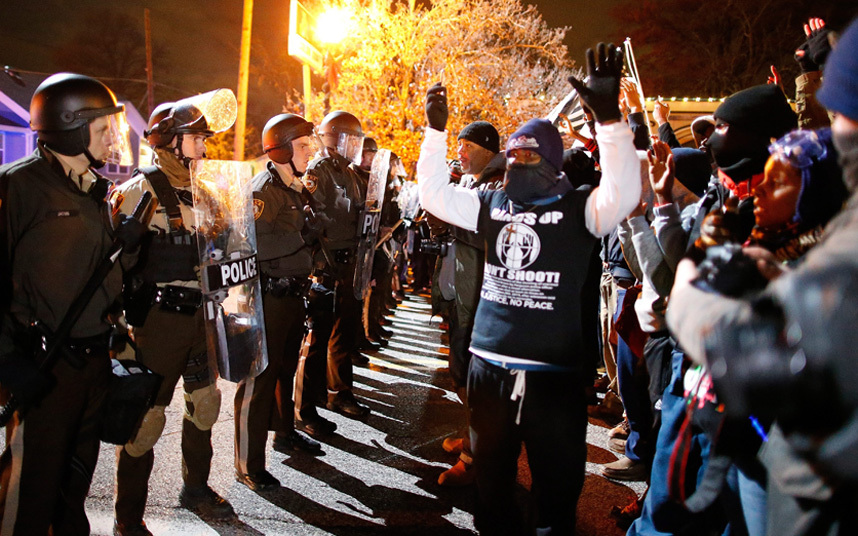
\includegraphics[width=8cm]{images/photos/ferguson_riots.jpg}
\caption{Photo of the Ferguson riots. On the left, policemen, on the right, protesters raising hands and saying "Don't Shoot"}
\vspace*{-1cm}
\end{wrapfigure}

On August 9th, 2014, a 18-year-old black man called Michael Brown is shot dead in Ferguson by a white police officer. This event was the trigger of riots, both peaceful and violent, for more than 2 weeks.

On November 24th, the Grand Jury decides not to indict the police officier who shot dead Michael Brown, sparking unrest in Ferguson and in others cities accross the US, like in Boston or Los Angeles.



As for former unrest, the Ferguson protest has been widely broadcasted on social medias like Twitter. 

Some people, like Antonio French, were particularly active. Although not being a journalist, but leaving near Ferguson, he reported daily through Twitter what was happening in the field.
\begin{figure}[H]
\begin{subfigure}[t]{0.48\textwidth}
\begin{center}
	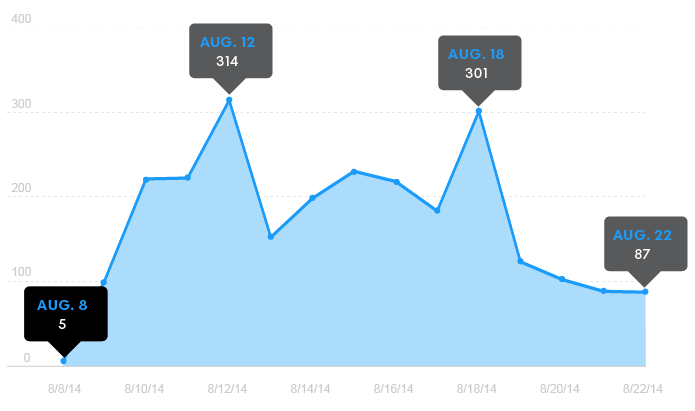
\includegraphics[width=\textwidth]{images/freqs/intro/af_tweets.png}
	\caption{Tweets count per day}
\end{center}
\end{subfigure}
\hfill
\begin{subfigure}[t]{0.48\textwidth}
\begin{center}
	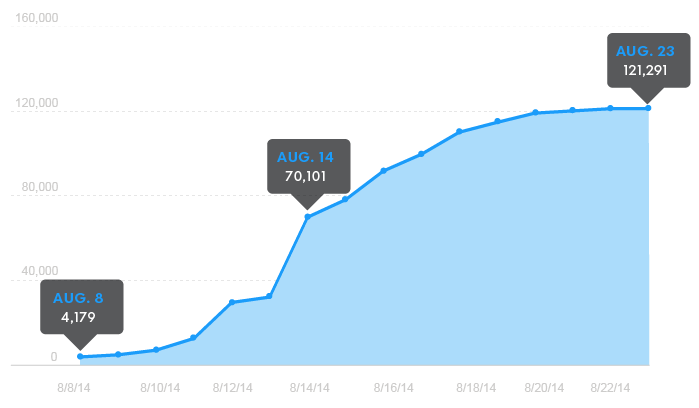
\includegraphics[width=\textwidth]{images/freqs/intro/af_followers.png}
	\caption{Followers cumulative count per day}
\end{center}
\end{subfigure}
\caption{Antonio French's activity during the protest (\copyright \texttt{ usatoday.com})}
\label{afactivity}
\end{figure}
One can see on the figure \ref{afactivity} how Antonio French was active (up to 300 tweets a day) during the whole unrest. And, even more interesting, the figure shows how he became popular, as he was followed by more than 120,000 people at the end of the protest, whereas he was almost unknown on Twitter before. 

As the article shows through example tweets, Antonio French had an informative role. He mostly posted pictures and videos during each riot, and everytime, he tried to gather information about what was happening.\\
In this way, it is interesting to wonder:
\begin{itemize}
\vspace*{-0.2cm}
\setlength\itemsep{0em}
\item How to model such a role on Twitter during a riot ?
\item How to say if two users are similar ?
\item How to group users given the role they play ?
\item How to visualize this kind of information ?
\end{itemize}

The following part describes the problem and the objectives more formally.
\newpage

\section{Formulation and objectives}

In this part we introduce clearly the objectives this project will try to fulfil. \\
Firstly, we define and formulate three entities : a \textbf{protest}, a \textbf{riot} and a \textbf{topic}.

\begin{defbox}
\textbf{Definition} - Protest $\mathcal{P}_n$\\
A protest $\mathcal{P}_n$ is defined as a time ordered list of $n$ riots $r$.
$$ \mathcal{P}_n = [r_1, r_2, \cdots, r_n]$$
In our case, we suppose there is a riot each night. As a consequence, $\mathcal{P}_n$ is $n$-days long.
\end{defbox}

\begin{defbox}
\textbf{Definition} - Riot $r$ and topics $t$\\
A riot $r$ is defined as a set of $m$ topics $t$ occuring during the riot $r$.
$$ r = [t_1, t_2, \cdots, t_n]$$
\end{defbox}
The main objective of this project is given by :

\begin{objbox}\color{Maroon}
\textbf{Main Objective} : Define and compute the \textbf{role} of a user, the similarity between two users and clusters these users by their role.
\end{objbox}

We decide to characterize the role of a user by a simple model with two features :
\begin{itemize}
\item \textbf{Polarity}. What kind of content does the user publish ? How to characterize it ? What are the different types of content existing ? How to quantify it ?
\item \textbf{Influence}. Does the user has influence ? How to quantify it? How to visualize it ? How does this influence evolve ?
\end{itemize}
This leads to two intermediary objectives : 
\begin{objbox}\color{Maroon}
\textbf{Objective 1.} Define and compute the \textbf{polarity} of a user.
\end{objbox}

\begin{objbox}\color{Maroon}
\textbf{Objective 2.} Define and compute the \textbf{influence} of a user.
\end{objbox}

\newpage

\section{Technical details}
All the code has been written in Python and uses the following libraries : 
\begin{itemize}
\item \textbf{NLTK}, for the Natural Language Processing part ;
\item \textbf{Scikit-Learn}, for the machine learning algorithms ;
\item \textbf{Gensim}, for the topic modeling part ;
\item \textbf{Networkx}, for creating and manipulating graphs ;
\end{itemize}

The code is hosted on Github at the following url :
\begin{center}
\vspace{0cm}
\url{http://github.com/jwheatp/twitter-riots}
\end{center}

The computation tasks have been made on the Linux Ubuntu \texttt{brute.aalto.fi} server, model HP BL460c.
%%%%%%%%%%%%%%%%%%%%%%%%%%%%%%%%%%%%%%%%%%%%%%%%%%%%%%%%%%%%%%%%%%%%%%%
%%%%%%%%%%%%%%%%%%%%%%%%%%%%%%%%%%%%%%%%%%%%%%%%%%%%%%%%%%%%%%%%%%%%%%%
%%%%%% CHAPTER 2 - DATASET
%%%%%%%%%%%%%%%%%%%%%%%%%%%%%%%%%%%%%%%%%%%%%%%%%%%%%%%%%%%%%%%%%%%%%%%
%%%%%%%%%%%%%%%%%%%%%%%%%%%%%%%%%%%%%%%%%%%%%%%%%%%%%%%%%%%%%%%%%%%%%%%

\chapter{Dataset}

\section{Origin}
The choice of the Ferguson riots as a case study has been made for several reasons. Firstly, this is a recent case, as it occured last year. Moreover, this events happened in a country that use social medias a lot. In addition, the fact all the tweets are in English makes the study of the language easier than studying, for example, the Arab Spring protests. But one of the main reason was that this dataset was available.

Indeed, obtaining datasets about riots is not a simple task. Twitter does not allow to fetch past tweets between two dates with a precise keyword, but only new tweets from the Stream API. Some research groups manage to grant a special access from Twitter, like for the London riots study\cite{procter2013reading}, but do not make these datasets publicly available online.

Moreover, Twitter does not allow neither peers to share full datasets obtained with its API. However, the company allows people for now to share IDs list of tweets, without any content. One is then able to use the Twitter API to fetch, for each ID, the tweet content (text, author, date etc.) under the rates limitations.

The dataset used in this project is obtained from Ed Summers, a developer who started to record the Ferguson-related tweets after Mike Brown's shooting and who published on his blog the IDs list\footnote{\url{http://inkdroid.org/journal/2014/08/30/a-ferguson-twitter-archive/}}. The task was then to \emph{hydrate} the tweets and users to obtain the full dataset.

Contrary to a more advanced (and therefore costly) tool called Firehorse, the free Stream API allow developers to fetch only $1\%$ of the live stream. In other ways, considering all the tweets published at the present moment, one is able with the Stream API to get only $1\%$ of the total tweets. But does this $1\%$ sample is \emph{representative} of all published content ? Studies \cite{DBLP:journals/corr/MorstatterPLC13} and \cite{morstatter2014biased} demonstrates that even if biases can be introduced, the sample data remains close and representative to the all stream.

In order to collect the data, the Twitter Stream API has been used with the keyword Ferguson between the August 10th and 27th. As a consequence, every tweet containing this word (not only hashtag) and present in the sample stream during that period is present in our dataset. In the end, our dataset contains approximately 12 million tweets.

\newpage

\section{Structure}
The dataset contains approximately 12 million tweets and contains data from August 10th to August 27th. In this part we describe a tweet and a user and their structures.

\subsection{Tweet structure}
A \textbf{tweet} represents a message a user posted and its metadatas, like the publication date, its identification number, a media (photo / link) etc. Some metadatas are specific to Twitter : 
\begin{itemize}
\item hashtag : represent a keyword in the message, written with the \# symbol. It allows Twitter to classify tweets given their content.
\item mention : represent a reference to another user in the message, written with the @ symbol. It is commonly used so people can talk each other.
\end{itemize}
There are special tweets called \emph{retweets}. They start by \texttt{RT @user} and allow a user to share a tweet of another user. A tweet with an important retweet count is considered as popular

The detailed structure of a tweet is given on figure \ref{structTweet}.

\begin{figure}[h!]
\centering
\begin{tabular}{ccc}
field & type & example\\
\hline
\hline
id & number & \texttt{498619822134280192} \\ \hline
publication date & date & \texttt{2014-08-11 00:00:04} \\ \hline
author id & number & \texttt{124010717} \\ \hline
text & number & \pbox{9cm}{\vspace*{5pt}\texttt{Please follow @AntonioFrench now! \newline \#Ferguson \#MikeBrown http://t.co/---}\vspace*{5pt}} \\ \hline
retweet count & number & \texttt{4} \\ \hline
is it a retweet ? & boolean & \texttt{False} \\ \hline
hashtags & string list & \texttt{\#Ferguson, \#MikeBrown} \\ \hline
mentions & string list & \texttt{@AntonioFrench} \\ \hline
links and medias & string list & \texttt{http://t.co/---} \\ \hline \hline
\end{tabular}
\caption{Structure of a tweet}
\label{structTweet}
\end{figure}

\newpage

\subsection{User structure}
A \textbf{user} represents a person or an organization. They can be properly named with the real full name of the author or just use a nickname. In addition, a user has an identification nickname, usually short, that is used for mentions in a message, as described above. A user can follow and be followed by people. Contrary to social medias as Facebook, he the links are unidirectional. If user $A$ follows user $B$, user $B$ may not follow user $A$. A user with an important followers count is considered as popular.

The detailed structure of a user is given on figure \ref{structUser}.

\begin{figure}[h!]
\centering
\begin{tabular}{ccc}
field & type & example\\
\hline
\hline
user id & number & \texttt{14090948} \\ \hline
name & string & \texttt{Antonio French} \\ \hline
nickname & string & \texttt{AntonioFrench} \\ \hline
registration date & date & \texttt{2008-03-06 19:51:29} \\ \hline
tweet count & number & \texttt{19372} \\ \hline
followers count & number & \texttt{119977} \\ \hline
friends count & number & \texttt{1373} \\ \hline \hline
\end{tabular}
\caption{Structure of an user}
\label{structUser}
\end{figure}


\newpage

\section{Basic analysis}

\subsection{Frequencies}
\label{subSecFreqs}
We compute the hour-frequency of tweets, that is to say the number of tweets published every hour for each day. The result is shown on figure \ref{freqTweets}. We distinguish several kinds of tweets : 
\begin{itemize}
\item \textbf{tagged} : tweets containing a least one hashtag, \underline{except} the two most popular that are \texttt{\#Ferguson} and \texttt{\#MikeBrown}.
\item \textbf{min-tagged} : tweets containing a least one hashtag, \underline{including} the two most popular that are \texttt{\#Ferguson} and \texttt{\#MikeBrown}.
\item \textbf{no-tagged} : tweets with no hashtag at all
\item \textbf{retweets} : only retweets, no simple tweets.
\item \textbf{total} : all the tweets
\end{itemize}

Firstly, one can see the frequencies distribution. We clearly have peaks of frequency during the nights, from midnight to the morning. This corresponds to the riots happening during the nights.

Moreover, one can notice the hashtags proportions. Approximately less than a half of the tweets (and sometimes only a third) contains non trivial hashtags (namely not \texttt{\#Ferguson} or \texttt{\#MikeBrown}). This raises the question of the relevance of studying hashtags in this situation.

In addition, the proportion of retweets is very high each day. This means that most of the people just retweet relevant content instead of writing themselves.

\begin{figure}[H]
\begin{subfigure}[t]{0.48\textwidth}
\begin{center}
	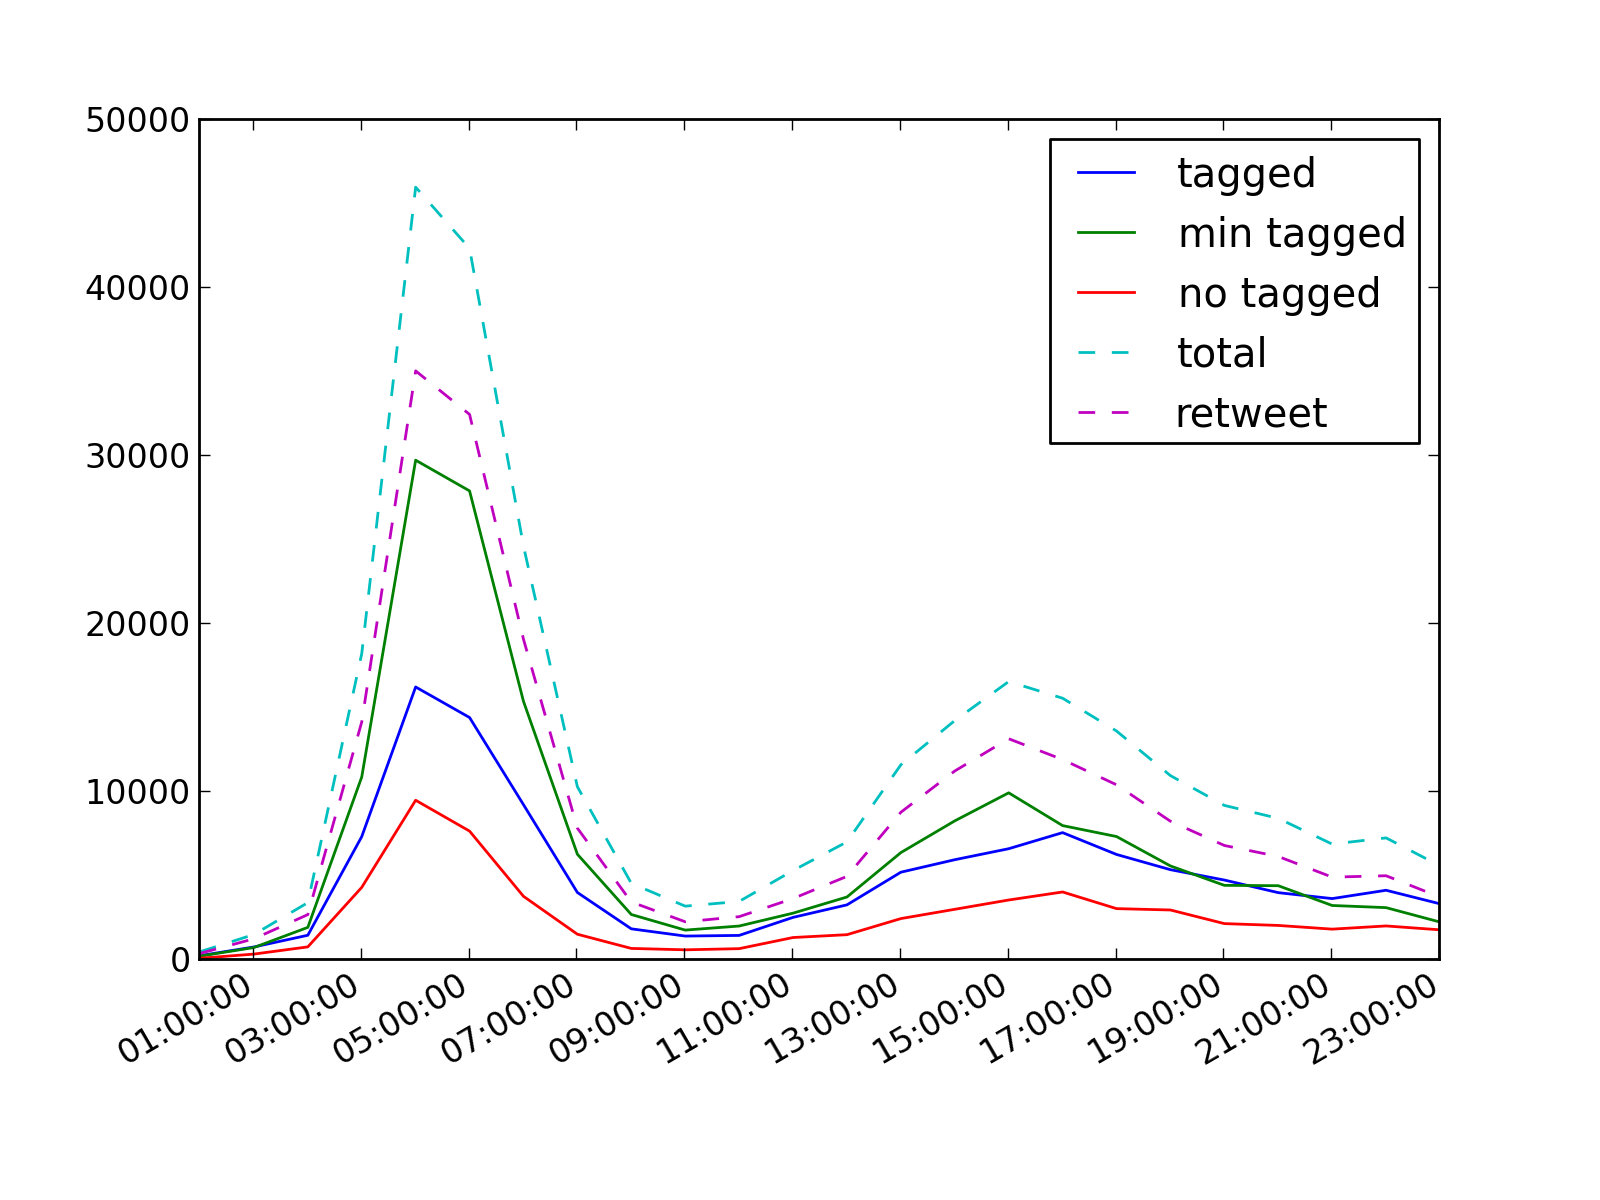
\includegraphics[width=\textwidth]{images/freqs/freq_11_08.png}
	\caption{August 11th}
\end{center}
\end{subfigure}
\hfill
\begin{subfigure}[t]{0.48\textwidth}
\begin{center}
	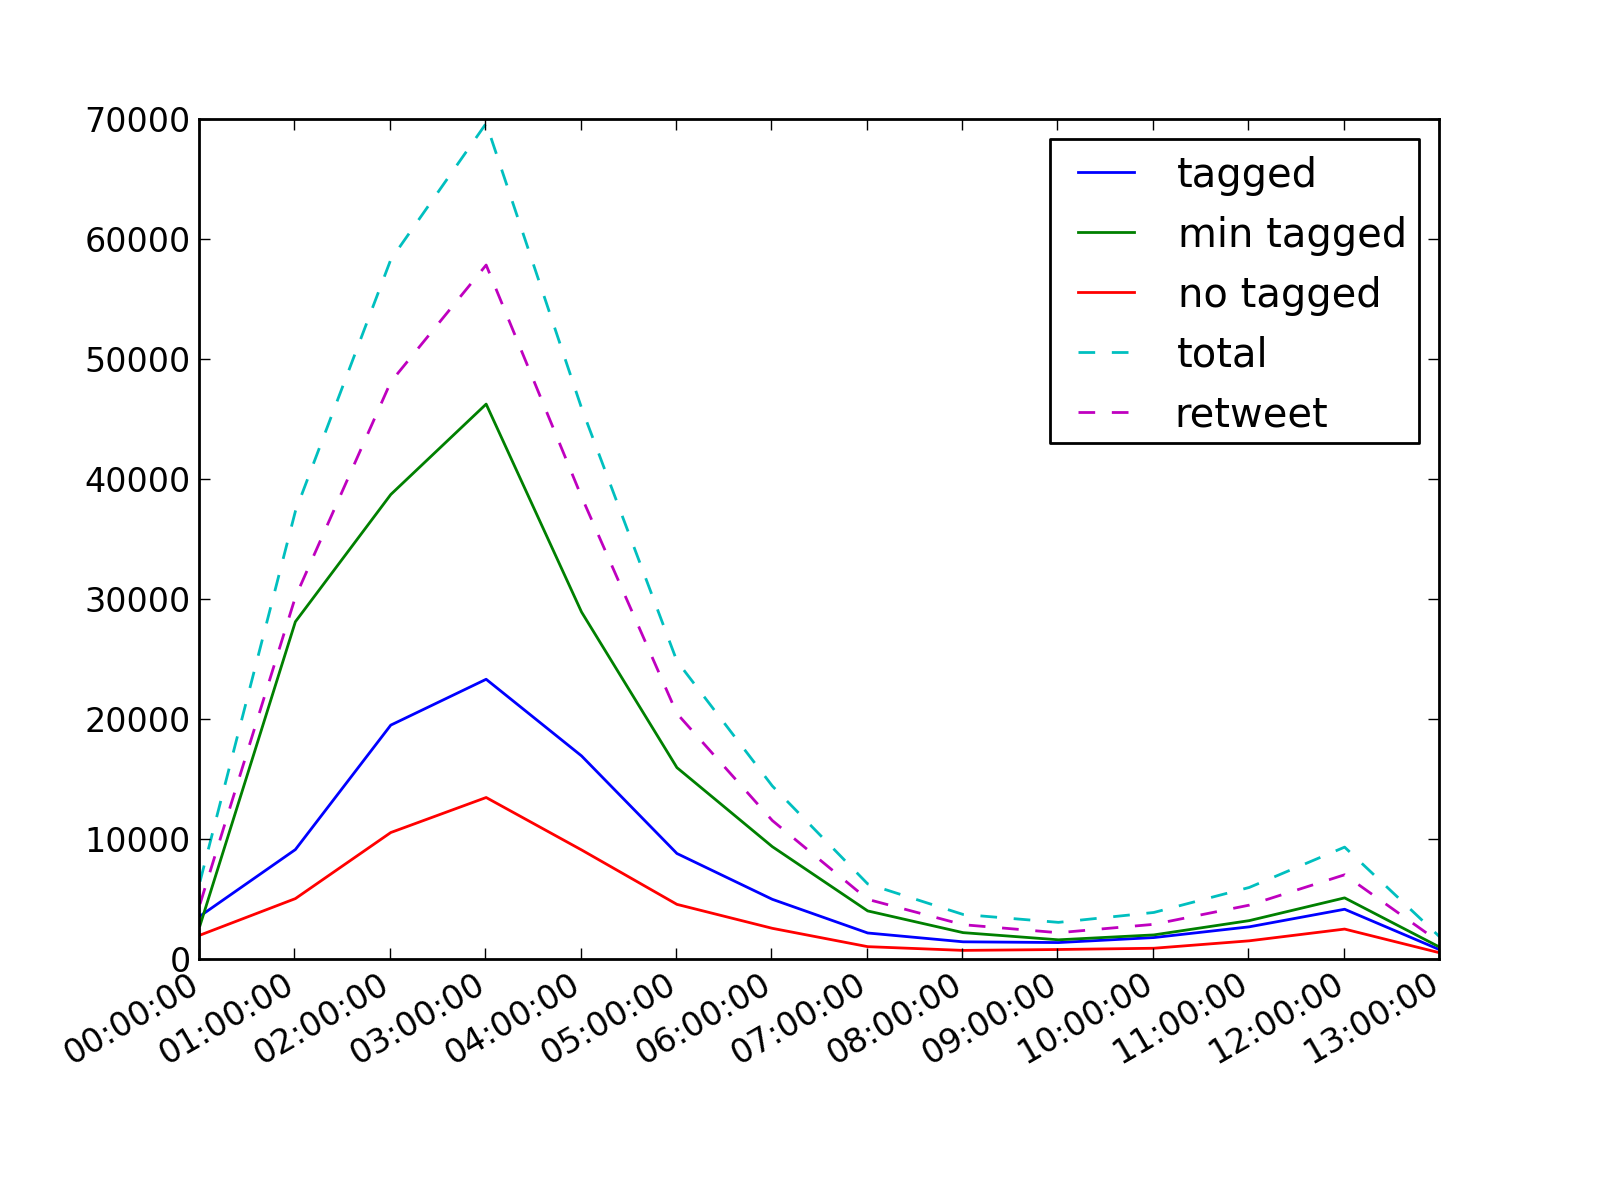
\includegraphics[width=\textwidth]{images/freqs/freq_12_08.png}
	\caption{August 12th}
\end{center}
\end{subfigure}

\begin{subfigure}[t]{0.48\textwidth}
\begin{center}
	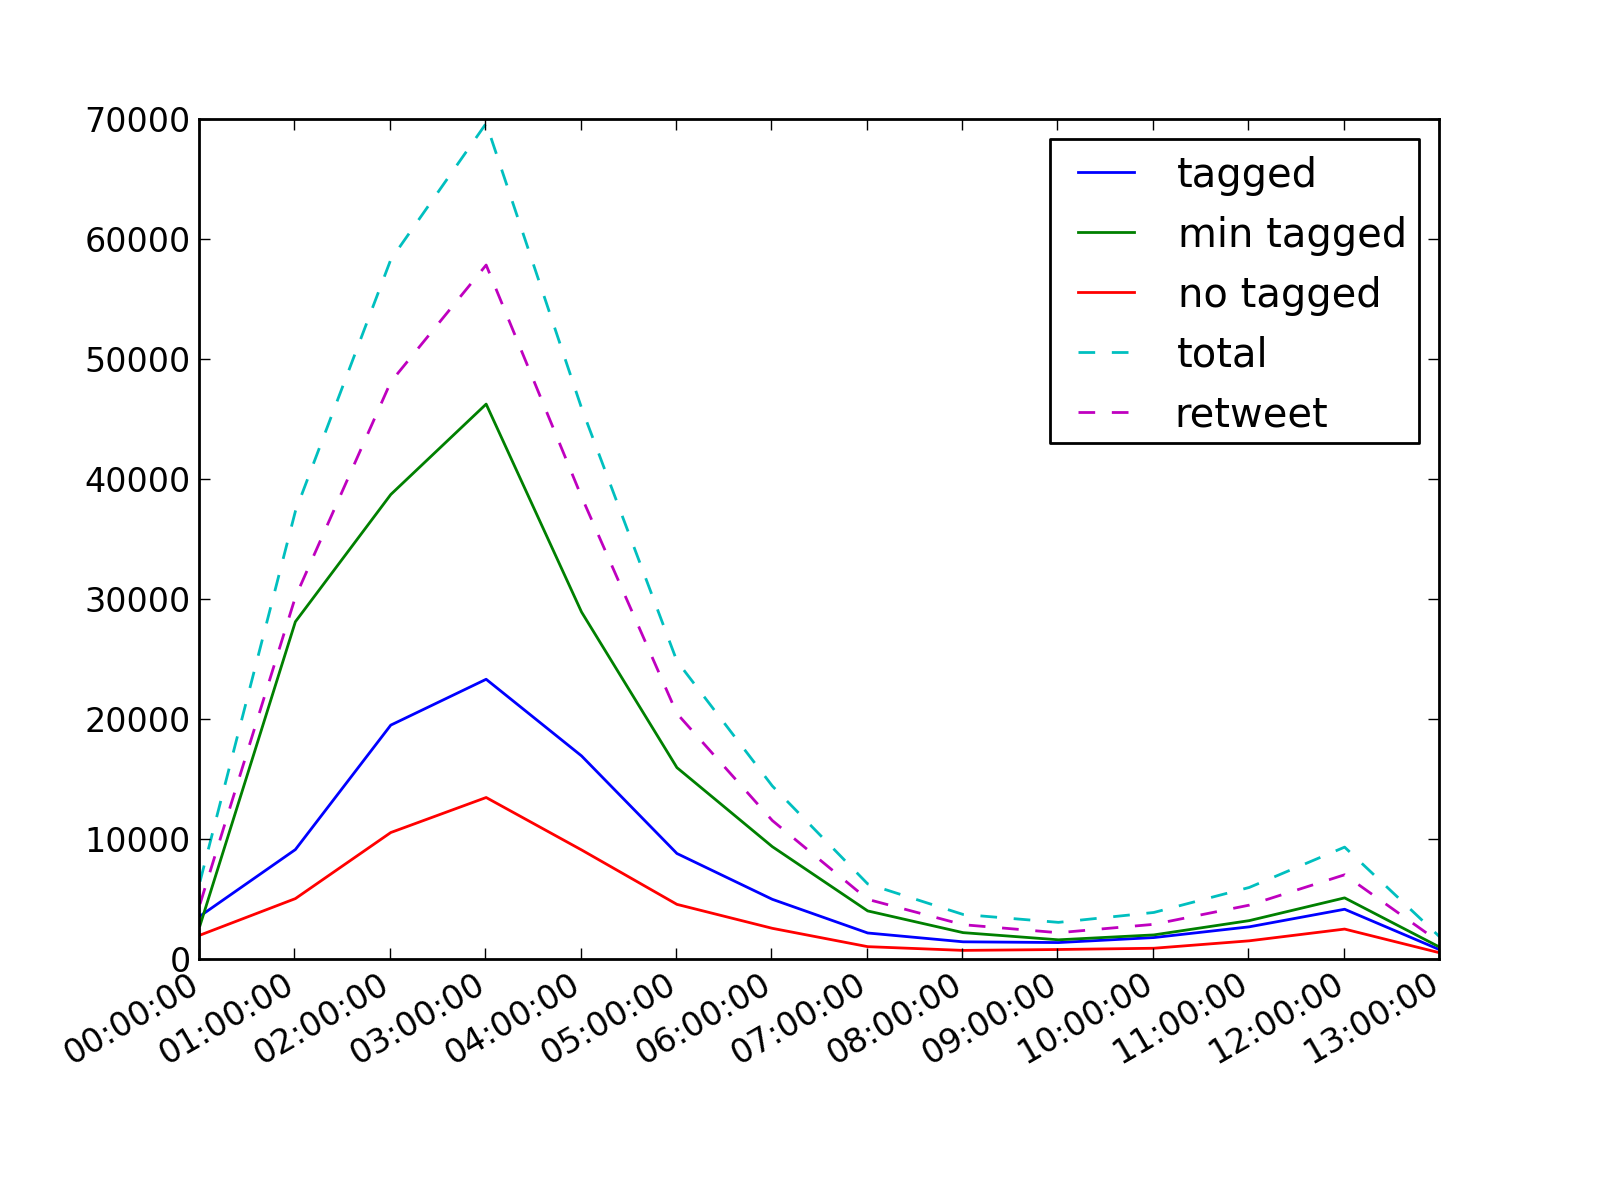
\includegraphics[width=\textwidth]{images/freqs/freq_12_08.png}
	\caption{August 13th}
\end{center}
\end{subfigure}
\hfill
\begin{subfigure}[t]{0.48\textwidth}
\begin{center}
	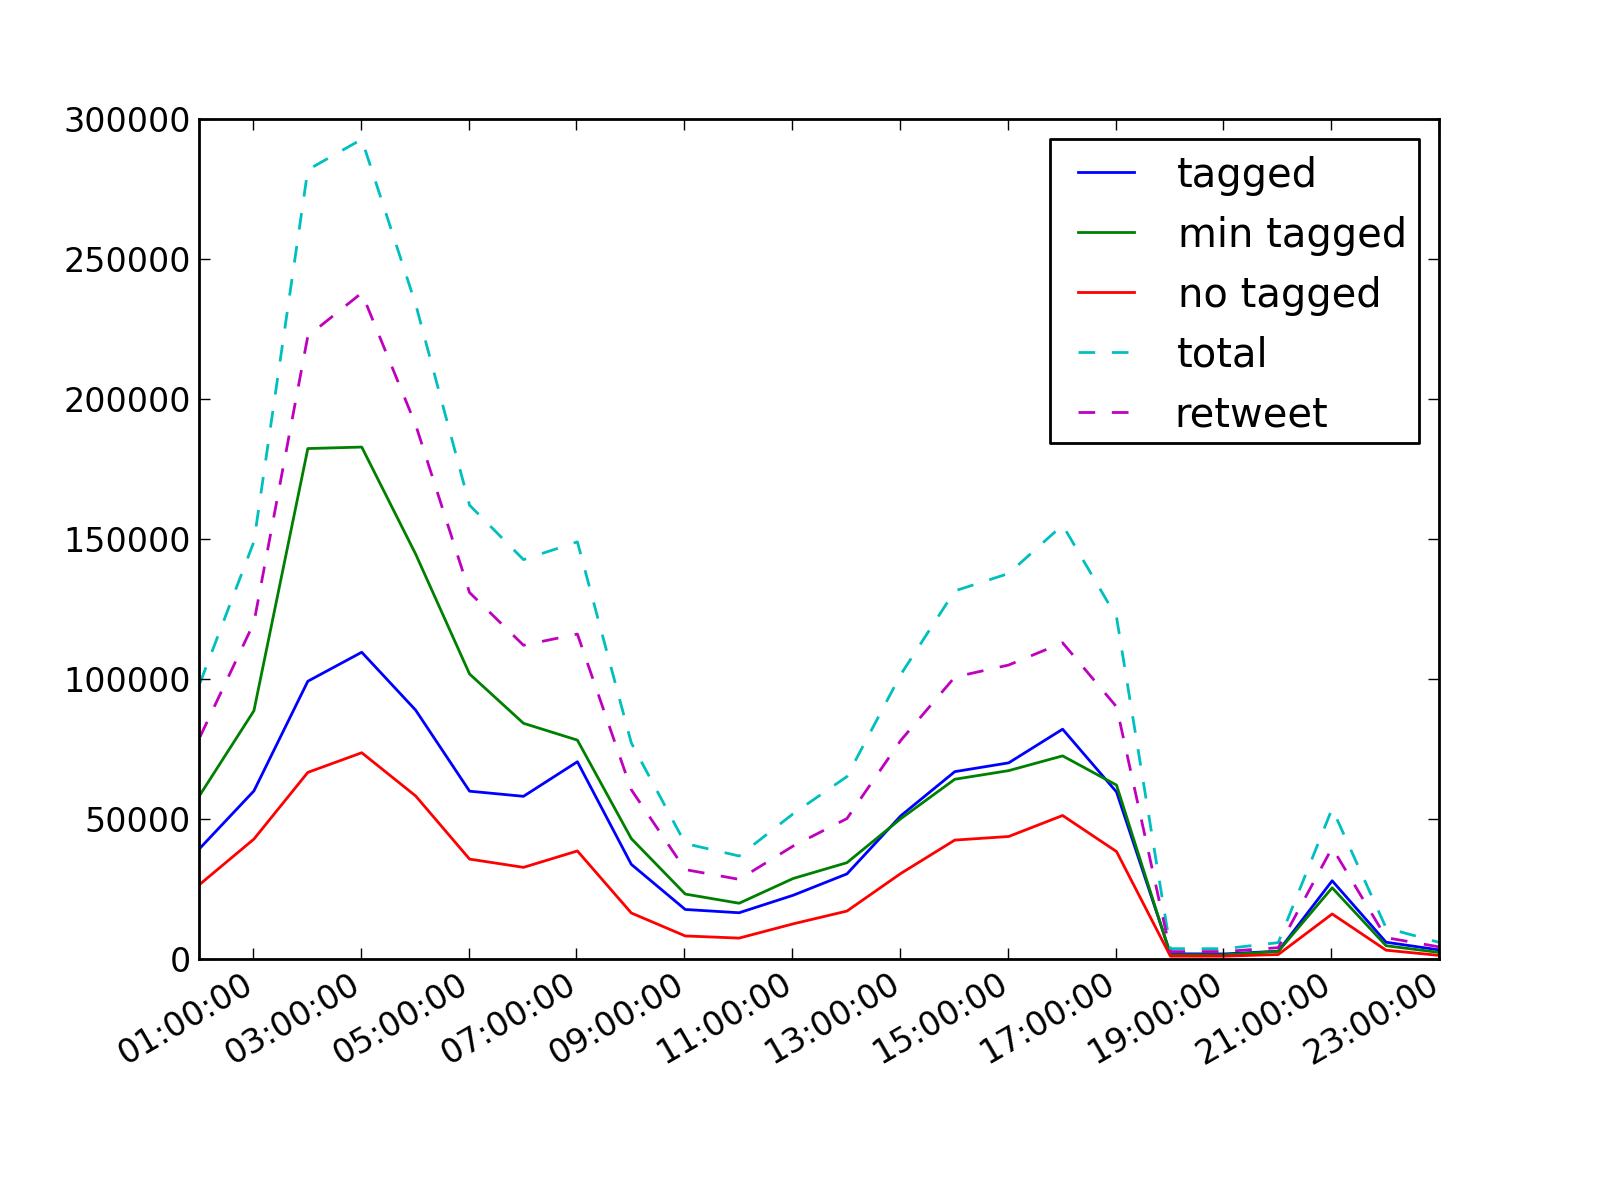
\includegraphics[width=\textwidth]{images/freqs/freq_14_08.png}
	\caption{August 14th}
\end{center}
\end{subfigure}

\begin{subfigure}[t]{0.48\textwidth}
\begin{center}
	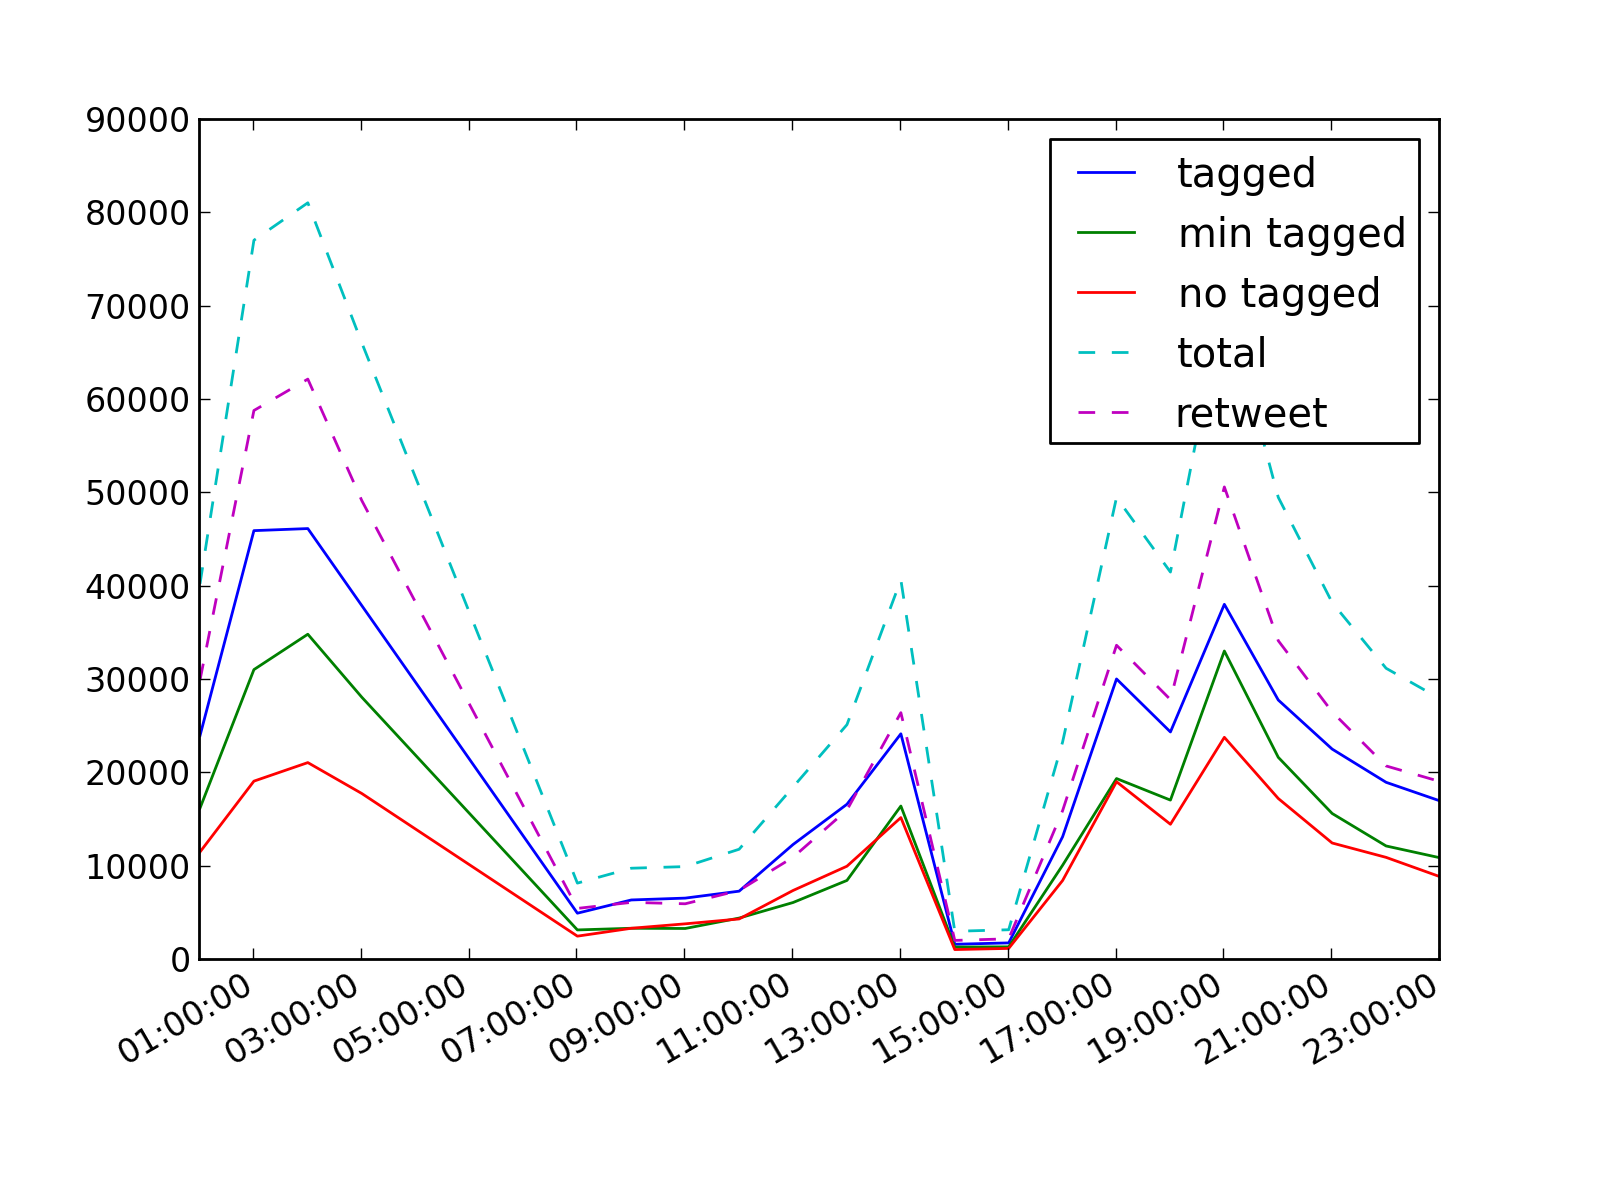
\includegraphics[width=\textwidth]{images/freqs/freq_15_08.png}
	\caption{August 15th}
\end{center}
\end{subfigure}
\hfill
\begin{subfigure}[t]{0.48\textwidth}
\begin{center}
	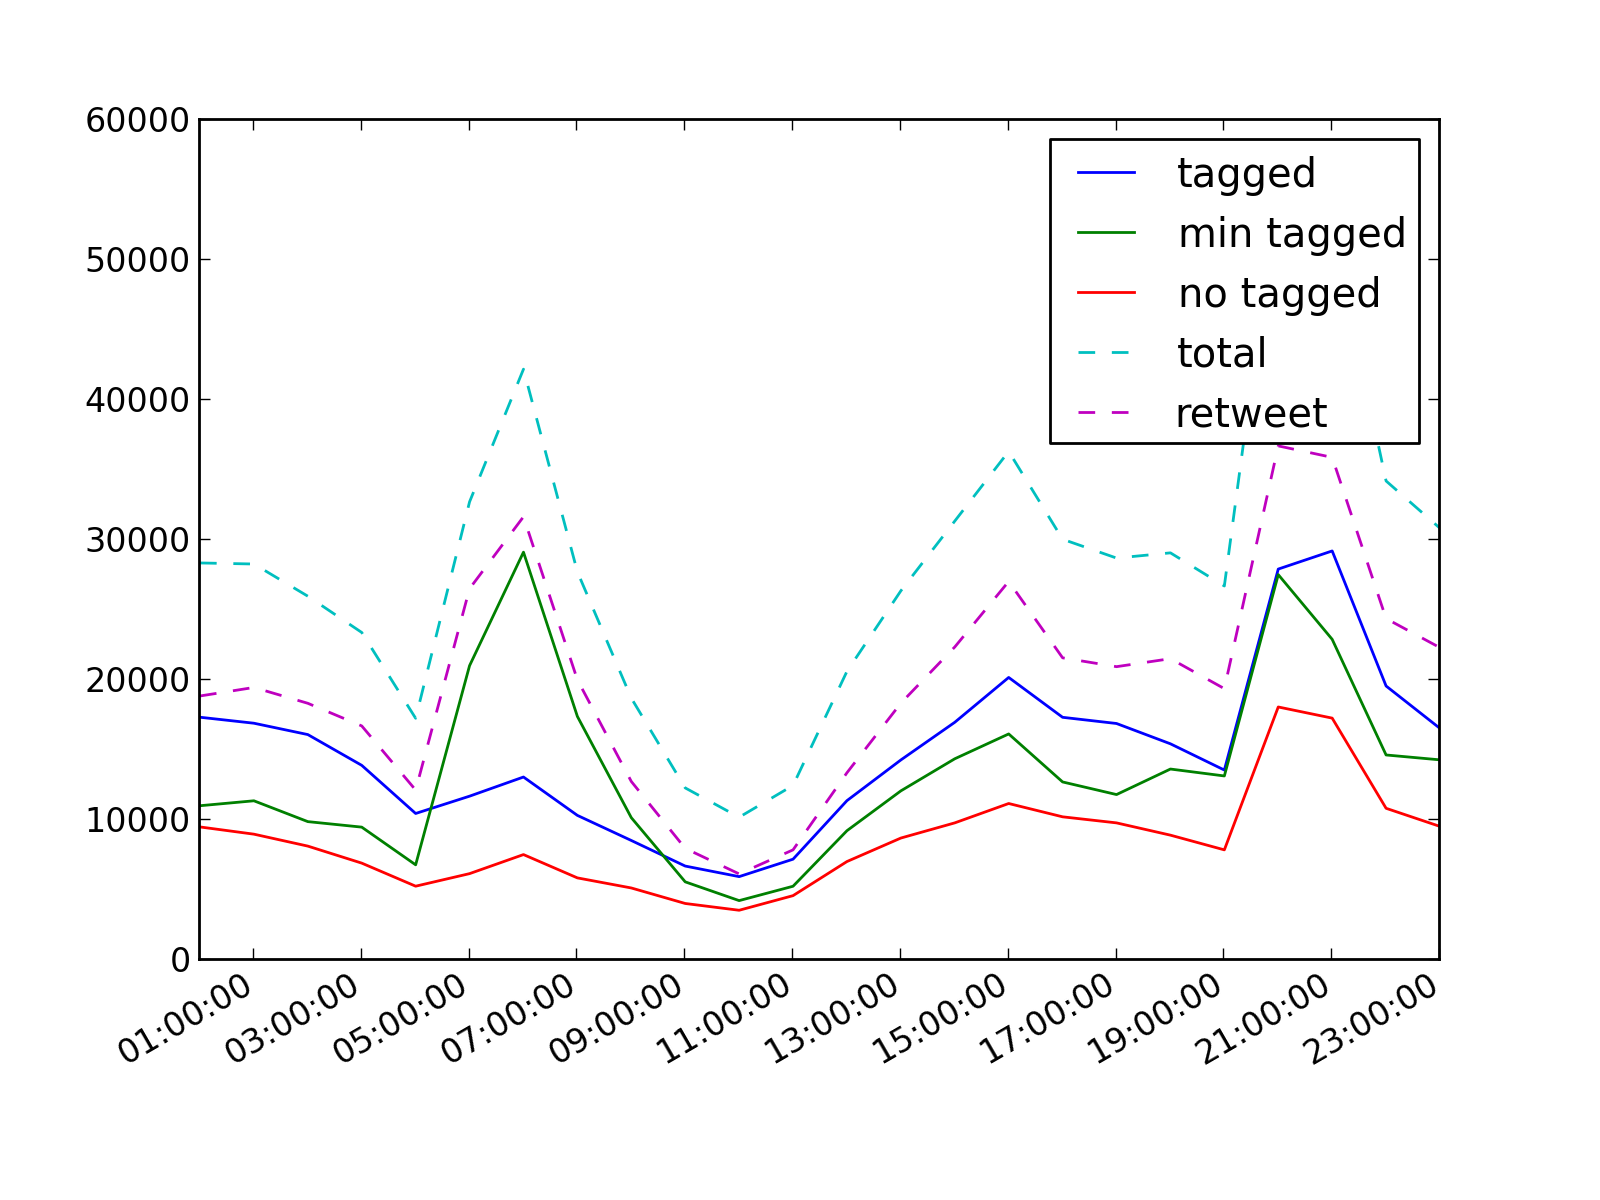
\includegraphics[width=\textwidth]{images/freqs/freq_16_08.png}
	\caption{August 16th}
\end{center}
\end{subfigure}
\caption{Tweets frequencies}
\label{freqTweets}
\end{figure}

\newpage

\subsection{Most retweeted users}
In this section we take a look at the most retweeted users. These are the ones for which the tweets appear among the top 100 retweets for a considered day.

The figure \ref{activitiesPlots} show the most retweeted users for four days. For each plot, one can see the most retweeted users of the corresponding day and their activity evolution on the other days. For example, on figure \ref{activitiesPlots11}, the user \texttt{michaelskolnik} has 25 tweets appearing in the top 100. But we see that on the August 12 decreases to 3 tweets, and then he completely disappear. Some users like \texttt{antoniofrench} or \texttt{youranonnews} remains in the ranking almost for the six days.

On figure \ref{activitiesPlots16} that corresponds to the August 16, we notice that the user \texttt{ryanjreilly} appear in the rank on the August 15 and begin more popular day by day. Moreover, some users like \texttt{koranaddo} or \texttt{michaelcalhoun} appear to be popular for only one day.

This highlights different kind of popular users : 
\begin{itemize}
\item the users very popular at the begining but who disappear after several day, and on the contrary the users who are not popular for some days but appear in the ranking a given moment ;
\item the users who are only popular for a short moment, like a day ;
\item the users that stay popular and retweeted a lot all through the protest.
\end{itemize}

\begin{figure}[H]
\begin{subfigure}[t]{0.5\textwidth}
\begin{center}
	\includegraphics[width=\textwidth]{images/plots/influence/allfreqInluentUsers_11_08.png}
	\caption{August 11th}
	\label{activitiesPlots11}
\end{center}
\end{subfigure}
\hfill
\begin{subfigure}[t]{0.5\textwidth}
\begin{center}
	\includegraphics[width=\textwidth]{images/plots/influence/allfreqInluentUsers_14_08.png}
	\caption{August 14th}
	\label{activitiesPlots14}
\end{center}
\end{subfigure}

\begin{subfigure}[t]{0.5\textwidth}
\begin{center}
	\includegraphics[width=\textwidth]{images/plots/influence/allfreqInluentUsers_16_08.png}
	\caption{August 16th}
	\label{activitiesPlots16}
\end{center}
\end{subfigure}
\hfill
\begin{subfigure}[t]{0.5\textwidth}
\begin{center}
	\includegraphics[width=\textwidth]{images/plots/influence/allfreqInluentUsers_17_08.png}
	\caption{August 17th}
	\label{activitiesPlots17}
\end{center}
\end{subfigure}
\caption{Most retweeted users on diffent days}
\label{activitiesPlots}
\end{figure}

%\subsubsection*{0am-2am (2,058 tweets)}
%\toprt{top_rt_11_08_00_02}
%\subsubsection*{2am-4am (22,297 tweets)}
%\toprt{top_rt_11_08_02_04}
%\subsubsection*{4am-7am (113,264 tweets)}
%\toprt{top_rt_11_08_04_07}

%%%%%%%%%%%%%%%%%%%%%%%%%%%%%%%%%%%%%%%%%%%%%%%%%%%%%%%%%%%%%%%%%%%%%%%
%%%%%%%%%%%%%%%%%%%%%%%%%%%%%%%%%%%%%%%%%%%%%%%%%%%%%%%%%%%%%%%%%%%%%%%
%%%%%% CHAPTER 4 - DETECTING TOPICS
%%%%%%%%%%%%%%%%%%%%%%%%%%%%%%%%%%%%%%%%%%%%%%%%%%%%%%%%%%%%%%%%%%%%%%%
%%%%%%%%%%%%%%%%%%%%%%%%%%%%%%%%%%%%%%%%%%%%%%%%%%%%%%%%%%%%%%%%%%%%%%%

\chapter{Topic modeling}

\section{Motivation}

Before modeling users by the roles they play, we must define the support of reference, that is to say, the events or topics that will characterize their role.

The simple approach is to consider a riot as a whole, but this has limits. Indeed, in this case we don't consider a subject but a time window, which is not very significant. For example, let's take two distinct events $A$ and $B$ happening the same day, and two users called $Alice$ and $Bob$. Let's suppose $Alice$ only tweets about the event $A$, and $Bob$ only about the event $B$, and let's imagine they write positive things about their respective events. It would be wrong, only by considering the two events occur the same day, to conclude that $Alice$ and $Bob$ have the opinion. We must be sure they talk about the same things before comparing them.

In this chapter, we want to group the tweets by what they are talking about that is to say their underlying topic. Of course, it is not possible to automatically capture the meaning of the tweets and find topics that way, but we can try to clusters the tweets based on the word they contains.

After some preprocessing, we try two methods in order to achieve this.


\newpage

\section{Preprocessing}

Before analyzing the data, it's essential to preprocess it. 

\subsection{Content preprocessing}

\fbox{
  \parbox{\textwidth}{\texttt{
\colorbox{red!20}{RT @kharyp:} How police treat white opencarry supporter vs an unarmed black teen. Wonder why? \colorbox{red!20}{\#MikeBrown} \colorbox{red!20}{\#Ferguson} \colorbox{red!20}{http://t.co/jG3hGJRAuC}
}
  }
}

\begin{enumerate}
\item \textbf{\underline{Cleaning} :} we remove all the non textual items : 
  \begin{itemize}
    \item mentions
    \item hashtags
    \item urls
  \end{itemize}
\fbox{
  \parbox{0.9\textwidth}{\texttt{
How police treat white opencarry supporter vs an unarmed black teen. Wonder why?}
  }
}
\item \textbf{\underline{Tokenization} :} breaks the sentence into a list of tokens, that can be words or symbols (punctuation). The tokens order is not considered anymore and a token can appear several time in the list.  \\[10pt]
\fbox{
  \parbox{0.9\textwidth}{\texttt{
how, police, treat, white, opencarry, supporter, vs, an, unarmed, black, teen, ., wonder, why, ?}
  }
}
\item \textbf{\underline{Punctuation and Stop words removing} :}  keeps only the valuable tokens by removing symbols and too common words like \emph{what}, \emph{and}, \emph{of} etc.\\[10pt]
\fbox{
  \parbox{0.9\textwidth}{\texttt{
police, treat, white, opencarry, supporter, vs, unarmed, black, teen, wonder}
  }
}
\item \textbf{\underline{Stemming} :} keeps the stem of words, such as for example \emph{unarmed} and \emph{unarm} will be the same token. This process reduces the vocabulary and allows to compare more easily token lists.\\[10pt]
\fbox{
  \parbox{0.9\textwidth}{\texttt{
police, treat, white, opencarry, supporter, vs, unarm\st{ed}, black, teen, wonder}
  }
}

\end{enumerate}

\newpage

\subsection{Tweet embedding}
\label{tweetEmbeddingSection}

The goal is to characterize a tweet by the words it contains, by using for example the bag-of-words representation.

However, this method has its limits. Indeed, it does not consider how a word is common or not inside the whole corpus of tweets. For example, the word "Ferguson" is not very useful to characterize a tweet as it is a very common word in the corpus.

Instead, it is preferable to compute the TF-IDF, for term frequency – inverse document frequency, particularly used in text mining.

It is defined as follow : 

$$tfidf = tf \times idf$$ 
where 
$tf$ is the frequency of the word in the considered document (tweet) and
$$idf = log \frac{|D|}{|\{d_j | t_j \in d_j\}|}$$
where $D = \{d_j | j\in R\} $ is the set of documents (tweets) and $|.|$ is defined as the size of the set.

In this way, for each word of a tweet, we take into consideration if this word is common in the dataset or not, and ajust its frequency accordingly. This method allows to bring out the uncommon words that may characterize a tweet.

We are now able to represent a tweet in the space of the vocabulary words $\mathcal{V}$ :

\[
\bordermatrix{~ & word_1 & word_2 & \cdots & word_n \cr tweet =  & tfidf_1 & tfidf_2 & \cdots & tfidf_n \cr}
\]

And all the tweets vectors generate the term matrix $\mathcal{M}$ :

\[
\bordermatrix{
~ & word_1 & word_2 & \cdots & word_n \cr 
tweet_1 & tfidf_{1,1} & tfidf_{1,2} & \cdots & tfidf_{1,n} \cr
tweet_2 & tfidf_{2,1} & tfidf_{2,2} & \cdots & tfidf_{2,n} \cr
\hspace{10pt} \vdots & \vdots & \vdots & \ddots & \vdots \cr
tweet_m & tfidf_{m,1} & tfidf_{m,2} & \cdots & tfidf_{m,n} \cr
}
\]

\newpage

%\section{Distance between two tweets}

%\subsection{Euclidean distance}
%In order to evaluate if two tweets are close or not, distance functions.\\
%we need a distance function $\mathcal{D}$ such that
%$$ \mathcal{D} : X\times X \rightarrow \textbf{\textsf{R}}^+ $$
%and such that $\mathcal{D}$, for all $t_1$,$t_2$ $\in X$
%\begin{itemize}
%\item $\mathcal{D}(t_1,t_2)$ is \textbf{small} if $t_1$ and $t_2$ are \textbf{similar}
%\item $\mathcal{D}(t_1,t_2)$ is \textbf{large} if $t_1$ and $t_2$ are \textbf{dissimilar}
%\end{itemize}
%the most commonly used distance define as follow :
%$$ \forall t_1,t_2 \in X, \mathcal{D}(t_1,t_2) = || t_1 - t_2 ||_2 $$
%\subsection{Cosine similarity}
%we need a similarity function $\cos$ such that
%$$ \cos : X\times X \rightarrow \textbf{\textsf{R}}^+ $$
%and such that $\cos$, for all $t_1$,$t_2$ $\in X$
%\begin{itemize}
%\item $\cos(t_1,t_2)$ is \textbf{small} if $t_1$ and $t_2$ are \textbf{dissimilar}
%\item $\cos(t_1,t_2)$ is \textbf{large} if $t_1$ and $t_2$ are \textbf{similar}
%\end{itemize}
%$$ \forall t_1,t_2 \in X, \cos(t_1,t_2) = \frac{t_1.t_2}{||t_1||.||t_2||} $$

\newpage
\section{Clustering using $k$-means}

\subsection{$k$-means algorithm}
Given a set of documents $\mathcal{C} = \{d_1,d_2,\cdots,d_m\}$, we want to find $k$ centers, or topics, $t_1,t_2,\cdots,t_k$ that minimizes the cost :
$$ \sum_{i=1}^n \min_j ||d_i-t_j||_2^2 $$


\begin{algorithm}
\caption{$k$-means algorithm}
\label{algo:kmeans}
\begin{algorithmic} 
\STATE pick randomly $k$ center ${t_1,t_2,\cdots,t_k}$
\REPEAT
\STATE assign each point $d$ to its closest center t, in order to create $k$ clusters
\STATE compute the new centers by taking the mean of each cluster
\UNTIL{convergence}
\end{algorithmic}
\end{algorithm}

For a better initialization, some improved algorithms like $k$-means++ exist.

\subsection{Topic modeling}

After perfoming the $k$-means algorithm, we get two outputs : 
\begin{itemize}
\item the \textbf{tweets clusters}, that is to say each tweet belongs to one cluster that correspond to a topic.
\item the \textbf{topics}, that are the clusters centers. These are computed ``mean" tweets from the tweets belonging to each cluster.
\end{itemize}

\newpage 

\subsection{Experiment}
We experiment $k$-means on two riot days : the August 11 (figure \ref{topicKmeans11}) and the August 12 (figure \ref{topicKmeans12}).

\begin{figure}[H]
\begin{subfigure}[t]{\textwidth}
  \centering
\begin{tabularx}{0.9\textwidth}{l}
\hline
huge police crowd louis site st county live west killed \\ \hline
right police family nike liquor dollar goods sight store looted \\ \hline
right happening family people fire walmart shots department news looted \\ \hline
omg looting burning fire photo wow quiktrip quicktrip damn ground \\ \hline
florissant police stationed west burglarized walmart businesses officer w chambers \\ \hline
quicktrip burning people mo prayers n tonight go black need \\ \hline
feed ktvi stream rioting watch live updates coverage news scanner \\ \hline
right police looting riot people photo gas riots news dont \\ \hline
police fired area firing near walmart officer shots chambers scanner \\ \hline
via whats happening dellwood rioting wow damn killed shit looting \\ \hline
\end{tabularx}
\caption{August 11}
\label{topicKmeans11}
\end{subfigure}
\begin{subfigure}[t]{\textwidth}
\vspace*{30pt}
  \centering
\begin{tabularx}{0.9\textwidth}{l}
\hline
right police riot get tear people via got told thats \\ \hline
protect police brutality watching people officers killing street moving allowed \\ \hline
steve aerial neck wooden walsh police tonight video shot pellet \\ \hline
leave good shot people resident media scene tonight right hope \\ \hline
woman police screams pregnant month slam im force nnht ground \\ \hline
force right police like scene looks another world sounds look \\ \hline
right police tear gas masks rubber bullets mist shooting stand \\ \hline
police area tv media trapped turned leave lot ordered told \\ \hline
right police dont people media scene cops go home happening \\ \hline
via police qt media outside stay protest right today happened \\ \hline
\end{tabularx}
\caption{August 12}
\label{topicKmeans12}
\end{subfigure}
\caption{Topics obtained with $k$-means}
\end{figure}

\newpage
\section{Latent Dirichlet Allocation}
\label{LDASec}

\subsection{LDA algorithm}

\begin{center}
\begin{tabular}{ll}
Topics & $ \mathcal{T} = \{t_1,t_2,\cdots,t_k\} $ \\
Documents & $ \mathcal{C} = \{d_1,d_2,\cdots,d_m\} $ \\
Vocabulary & $ \mathcal{V} = \{w_1,w_2,\cdots,w_n\} $ \\
\end{tabular}
\end{center}

Let's consider that : 
\begin{enumerate}
\item each document is a probabilistic mixture of several underlying topics ;
\item each topic is a probabilistic distribution of words ;
\end{enumerate}

The topics are latent, hidden, as we do not observe them directly. They have to be infered from the words they are described with.

\subsubsection{Dirichlet distribution}
For three topics, the Dirichlet distribution for a document can be visualize in a triangle, as on figure \ref{diri_distri1}. Each corner represent a topic. The closer a document is to a corner, the higher is the probability that the document belongs to the topic. For example, on the figure \ref{diri_distri1}, the document belongs to the topic 2 with an higher probability than with the topics 1 and 3.

\begin{figure}[H]
\begin{minipage}[t]{0.48\textwidth}
\begin{center}
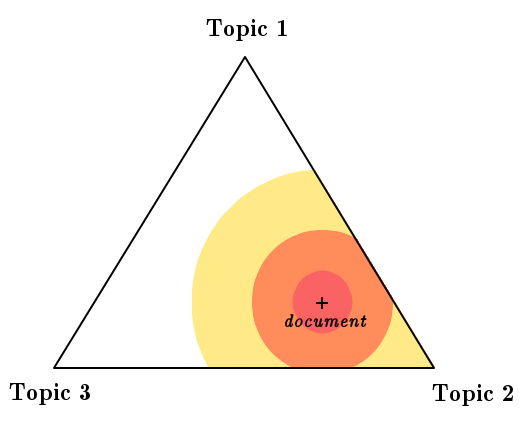
\includegraphics[width=\textwidth]{images/diags/lda_1.png}
\caption{Hashtag graph}
\label{diri_distri1}
\end{center}
\end{minipage}
\hfill
\begin{minipage}[t]{0.48\textwidth}
\begin{center}
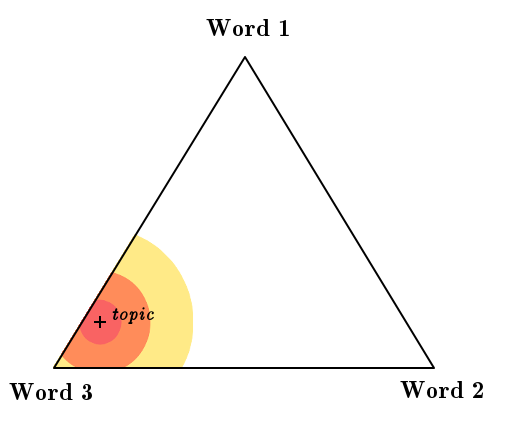
\includegraphics[width=\textwidth]{images/diags/lda_2.png}
\caption{Hashtag graph}
\label{diri_distri2}
\end{center}
\end{minipage}
\end{figure}

As figure \ref{diri_distri2} shows, we also have a Dirichlet distribution for the a topic and words (here 3 words). In this simple example, the topic is mostly characterized by the word 3, and a bit more by the word 1 than the word 2.

distribution of the topics $\beta$\\
topic proportions $\theta$\\

LDA follows the generate process : 
\begin{algorithm}
\caption{LDA : Generative process}
\label{algo:hashtagsGraph}
\begin{algorithmic} 
\FOR{each document $d$}
\STATE draw a distribution over topics $\theta_d \sim \textsf{Dirichlet}(\alpha)$
\FOR{each word $i$ in the document}
\STATE draw a topic $t$ in $\{t_1,\cdots,t_k\}$ according to $\theta_d$
\STATE draw the observed word $w$ according to $\beta_t$
\ENDFOR
\ENDFOR
\\[10pt]
\end{algorithmic}
\end{algorithm}

\subsubsection{Learning process}
The learning process consists of getting topics distributions and proportions according to the considered documents in the corpus.\\

// online learning algorithm 


\newpage

\subsection{Experiment}
We experiment LDA on two riot days : the August 11 (figure \ref{topicLDA11}) and the August 12 (figure \ref{topicLDA12}).

\begin{figure}[H]
\begin{subfigure}[t]{\textwidth}
  \centering
\begin{tabularx}{0.9\textwidth}{l}
\hline
racial profiling come shoot youth usa dont lessons survival black \\ \hline
right prayers language king unheard luther riot jr martin qt \\ \hline
praying officer police taco bell people swat news team pray \\ \hline
riots quiktrip today august watts ago began years burning tonight \\ \hline
quicktrip ground happening burning police looting gas tear wow scanner \\ \hline
photo burning quicktrip dogs community becomes police blame attention people \\ \hline
purge looting death mo people see guard via right police \\ \hline
police whats going nothing dellwood crazy difference changed pictures color \\ \hline
brown chaos looted police mike killed want looting shop oh \\ \hline
fired shots walmart live video fire police florissant looting quicktrip \\ \hline
\end{tabularx}
\caption{August 11}
\label{topicLDA11}
\end{subfigure}
\begin{subfigure}[t]{\textwidth}
\vspace*{30pt}
  \centering
\begin{tabularx}{0.9\textwidth}{l}
\hline
police gas tear officers stand riot masks protected mist live \\ \hline
n via historic tonight video protest like police st louis \\ \hline
nothing today get police home phones resident go happened thrown \\ \hline
police war missouri us shot riots city zone mo aerial \\ \hline
happening whats got going shit eyes need peace law news \\ \hline
media scene area pregnant leave told robin police williams thats \\ \hline
police people want dont black cops white watching street words \\ \hline
police violence shooting please journalists someone cars shut know anyone \\ \hline
right wow reporters gas tear photographers including bullets crowd rubber \\ \hline
jesus brown mike wow twitter pd obama time alex statement \\ \hline
\end{tabularx}
\caption{August 12}
\label{topicLDA12}
\end{subfigure}
\caption{Topics obtained with Latent Dirichlet Allocation}
\end{figure}


\newpage


\section{Comparison of the two methods}

Firstly, $k$-means is a \emph{hard-clustering} method, that is to say one tweet belongs to only one cluster (ie one topic) and the clusters are disjoint. 

On the contrary, LDA is a \emph{soft-clustering} method. The algorithm represent a tweet as a mixture of topics. As a consequence, with that model, a tweet can belongs to several topics with some probabilities.

Secondly, we can call into question the $k$-means approach essentialy because of the high-dimensionality of the vectors and their sparsity. Indeed, it is hard to evaluate if two vectors are close in a such voluminous space (for example with a vocabulary of 1000 words) especially as many components are equal to zero (as a tweet contains at most 140 characters).  Such dimensional problems will also be discussed in section \ref{dimReducSection}.

As a result, we choose to use the Latent Dirichlet Allocation method in the next of this project, as it seems to be the most realistic model.


%%%%%%%%%%%%%%%%%%%%%%%%%%%%%%%%%%%%%%%%%%%%%%%%%%%%%%%%%%%%%%%%%%%%%%%
%%%%%%%%%%%%%%%%%%%%%%%%%%%%%%%%%%%%%%%%%%%%%%%%%%%%%%%%%%%%%%%%%%%%%%%
%%%%%% CHAPTER 3 - CONTENT POLARITY
%%%%%%%%%%%%%%%%%%%%%%%%%%%%%%%%%%%%%%%%%%%%%%%%%%%%%%%%%%%%%%%%%%%%%%%
%%%%%%%%%%%%%%%%%%%%%%%%%%%%%%%%%%%%%%%%%%%%%%%%%%%%%%%%%%%%%%%%%%%%%%%

\chapter{Language analysis and content polarity}
\section{Motivation}
The main idea in this chapter is to characterize a user by what he writes in his tweets and in a general way we try to study the nature of the content shared by all the users during a riot.

Contrary to the previous chapter, we here tend to apply \emph{supervised learning} methods, that is to say we want to classify the tweets given an already existing classification of content types.

In the first part, we will establish a content type classification and we will build a model to predict it. In the second part, we will use the medias enclosed to the tweets in order to improve this model.

\newpage
\section{Characterizing tweets by their types}
In this section, we classify tweets by their nature. First, We establish a simple type classification below.

\subsection{Intuition}

\newcommand{\info}[1]{\colorbox{cyan!20}{#1}}
\newcommand{\rass}[1]{\colorbox{red!20}{#1}}
\newcommand{\ninfo}[1]{\colorbox{black!20}{#1}}
\newcommand{\nrass}[1]{\colorbox{green!20}{#1}}

By taking a look at some tweets obtained on the 11th of August, we can underline several types of tweets and construct the following classification :

\begin{figure}[h!]
\centering
\begin{tabular}{l|m{7cm}|m{6cm}}
type & details & example\\
\hline
\hline
\info{informative} & The tweet contains informative text content about the happening riot. The URL link is ignored. & ``\#Ferguson quiktrip burning http://t.co/1Jm5ngZe62" \\
\hline
\ninfo{non informative} & The tweet expresses feeling, an idea, a conviction, but no information about the happening riot. & ``Prayers for \#STL \#Ferguson." \\
\hline
\hline
\rass{involved} & The tweet support, encourages directly the happening riot, the rioters or their ideas. & ``Just spread the word we need \#Justice" \#ferguson \#stlouis \#MO  \#uniteblue \#libcrib \#p2 http://t.co/78QURveWvK" \\
\hline
\nrass{not involved} & The tweet is objective about the situation or blame the riot, the riotes or their ideas. & ``I am beyond saddened to see the looting in \#Ferguson. This removes the focus from justice for \#MikeBrown. Violence is never an answer." \\
\end{tabular}
\end{figure}

The figure \ref{tabtypes} shows more example of manually classified tweets. The second column highlights semantical or syntaxical details that helps to classify the given tweet.
One can notice the types pairs appearing, mostly :

\begin{itemize}
\item \info{informative}/\nrass{not involved} : tweets of interest as they are describing the riot situation in an objective way, for example eyewitnesses.
\item \ninfo{non informative}/\rass{involved} : useful tweets as their authors support the riot. It's interesting to consider the content in order to :
\begin{itemize}
\item understand the rioters claims ;
\item observe if the ``virtual violence" (language for example) of these users evolves ;
\item identify the main influencers.
\end{itemize}
\end{itemize}

The two others types are less interesting. Indeed, \ninfo{non informative}/\nrass{not involved} tweets does not contain any valuable information and \info{informative}/\rass{involved} tweets should be avoided as they may not contain objective information.

\newpage
\noindent
\begin{figure}[H]
\centering
\begin{tabular}{c|Cp{3cm}}
id & content & type \nl
1 & ``A riot is the language of the unheard." $~$Martin Luther King, Jr. \#Ferguson http://t.co/OXfzgEcN1B & \ninfo{non informative} \newline \nrass{not involved} \nl
2 & The Watts Riots began on \info{August 11, 1965}.  \info{49} years ago today. \#Ferguson http://t.co/gYgaI5WlP9 & \info{informative} \newline \nrass{not involved} \nl
3 & QuickTrip is \info{burning} to the ground. \#Ferguson http://t.co/9ykNn4a8ek & \info{informative} \newline \nrass{not involved} \nl
4 & \ninfo{Prayers} for \#STL \#Ferguson. & \ninfo{non informative} \newline \nrass{not involved} \nl
5 & The QuickTrip is \info{now} \info{burning}. \#Ferguson (photo: @PDPJ) http://t.co/tJBeXQ6hzF & \info{informative} \newline \nrass{not involved} \nl
6 & ``if you Retweet or Screenshot. Just \rass{spread the word} \rass{we need \#Justice}" \#ferguson \#stlouis \#MO  \#uniteblue \#libcrib \#p2 http://t.co/78QURveWvK & \ninfo{non informative} \newline \rass{involved}  \nl
7 & \info{Tear gas} is being used in \#Ferguson.  Mayor tells \info{CNN} he has been receiving death threats. \info{Armored vehicles roam the streets}. & \info{informative} \newline \nrass{not involved} \nl
8 & \rass{PAY ATTENTION} as "teen" becomes "man," "community" becomes "mob," and \rass{"murder" becomes "alleged shooting}." \#Ferguson \rass{\#medialiteracy} & \ninfo{non informative} \newline \rass{involved} \nl
9 & \info{Happening now} in \#Ferguson http://t.co/KFuaOEZ4tf & \info{informative} \newline \nrass{not involved} \nl
10 & \rass{Nothing has changed}. The ONLY difference?  The pictures are in color.  \#Ferguson \#FergusonShooting http://t.co/7p23qyDGwY & \ninfo{non informative} \newline \rass{involved} \nl
11 & \#Ferguson quiktrip \info{burning} http://t.co/1Jm5ngZe62 & \info{informative} \newline \nrass{not involved} \nl
12 & \info{Men} have \info{pulled} a \info{truck} up to the QT and are loading the ATM into the back. \#Ferguson & \info{informative} \newline \nrass{not involved} \nl
13 & \info{SWAT Team}. Taco Bell. \#Ferguson (photo:@kodacohen) http://t.co/Mo8CDVWx32 & \info{informative} \newline \nrass{not involved} \nl
14 & \info{Shots} \info{fired} at Walmart. \#Ferguson & \info{informative} \newline \nrass{not involved} \nl
15 & I am beyond saddened to \info{see the looting} in \#Ferguson. This removes the focus from justice for \#MikeBrown. \nrass{Violence is never an answer}. & \info{informative ?} \newline \nrass{not involved} \nl
\end{tabular}
\caption{Examples of maunal labeling}
\label{tabtypes}
\end{figure}

\newpage

\subsection{Multinomial Naives Bayes Classifier}

The model used is the Multinomial Naive Bayes, a well-used probabilistic learning method.
The Naive Bayes is a supervised method, which means its learns from a labelled dataset called training set. Once the model is trained, it can be used on unlabelled data. In order to measure the model accuracy, we run is on a test dataset.

\subsubsection{Naives Bayes}
Let $ \mathcal{D} = \{ d_i \}_{0\leq i\leq n} $ be the set of $n$ documents in the dataset.

For each document $d_i$, let $x_{1},x_{2},\cdots,x_{m}$ be its $m$ features, such as $$d_i = (x_{1},x_{2},\cdots,x_{m})$$
Let's assume the features are independent.

The probability that the document $d_i$ belongs to class $C_k$ is given by :
$$ P(C_k|d_i) = \frac{P(C_k)P(d_i|C_k)}{P(d_i)} $$
i.e. $$ P(C_k|x_{1},\cdots,x_{m}) = \frac{P(C_k)\prod_{j=1}^mP(x_{j}|C_k)}{P(d_i)} $$

The predicted class $\hat{C}$ is then given by the class that has the maximum probability :

$$ \hat{C} = \arg \max_k P(C_k|x_{1},\cdots,x_{m}) $$

\subsubsection{Word representation}

In our case, a document can be represented as a bag of words, which is a set where the word frequency is considered.

For example, given a document $d$ : \fbox{\texttt{prayers,mike,brown,prayers,ferguson}}

A bag-of-words representation would be :
\begin{center}
\begin{tabular}{|c|c|c|c|}
prayers & mike & brown & ferguson \\
2 & 1 & 1 & 1
\end{tabular}
\end{center}

Considering several documents as a dataset, we define the vocabulary $\mathcal{V}$ as the set of all the words existing in the dataset.

Continuing on the previous example, if $\mathcal{V}$ is defined as $\{\textsf{brown, ferguson, fire, mike, police, prayers, riots}\}$, the document $d$ can be represented as a count vector :

$$
\bordermatrix{~ & brown & ferguson & fire & mike & police & prayers & riots \cr d =  & 1 & 1 & 0 & 1 & 0 & 2 & 0 \cr}
$$

This is a multinomial document representation.

\subsubsection{Multinomial Naives Bayes}
The Multinomial Naives Bayes is a common variant for text classification.

$$ 
\boxed{P(x_{j}| C_k ) = \frac{N_{k,j} + \alpha}{N_k + \alpha n}}
$$

with 
\begin{itemize}
\item $N_{k,j}$ the count of the feature $x_j$ in the class $C_k$
\item $N_{k}$ the total count for all the features in $C_k$
\item $\alpha$ is a smoothing parameter, such that $\alpha \leq 1$, to avoid a zero value in the product of the naives bayes equation.
\end{itemize}


\subsubsection{Training the model}
In order to train our model, we manually label 500 tweets randomly choosen from the first riot (11 August). We annotate each document with two labels as follow : 

\begin{center}
\begin{tabular}{ccc}
informativness & involvement & ~ \\ \hline
0 & 0 & $\neg$ informative \& $\neg$ involved \\ \hline
0 & 1 & $\neg$ informative \& involved \\ \hline
1 & 0 & informative \& $\neg$ involved \\ \hline
1 & 1 & informative \& involved \\ \hline
\end{tabular}
\end{center}

One can see on figure \ref{screenshotLabeling} the manual labeling process. The script show a tweet message, and ask two \emph{boolean} questions : Is the tweet informative ? Is the tweet involved ?

\begin{figure}[H]
\centering
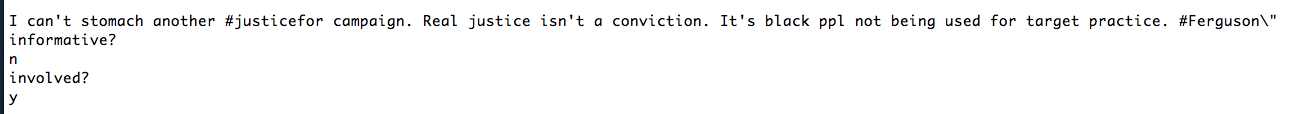
\includegraphics[width=\textwidth]{images/screens/manual_label_screen.png}
\caption{Screenshot of the manual labeling process}
\label{screenshotLabeling}
\end{figure}

\newpage

\begin{multicols}{2}[\textbf{Tweet type repartition on a manually classified 500 tweets sample}]

\begin{figure}[H]
\centering
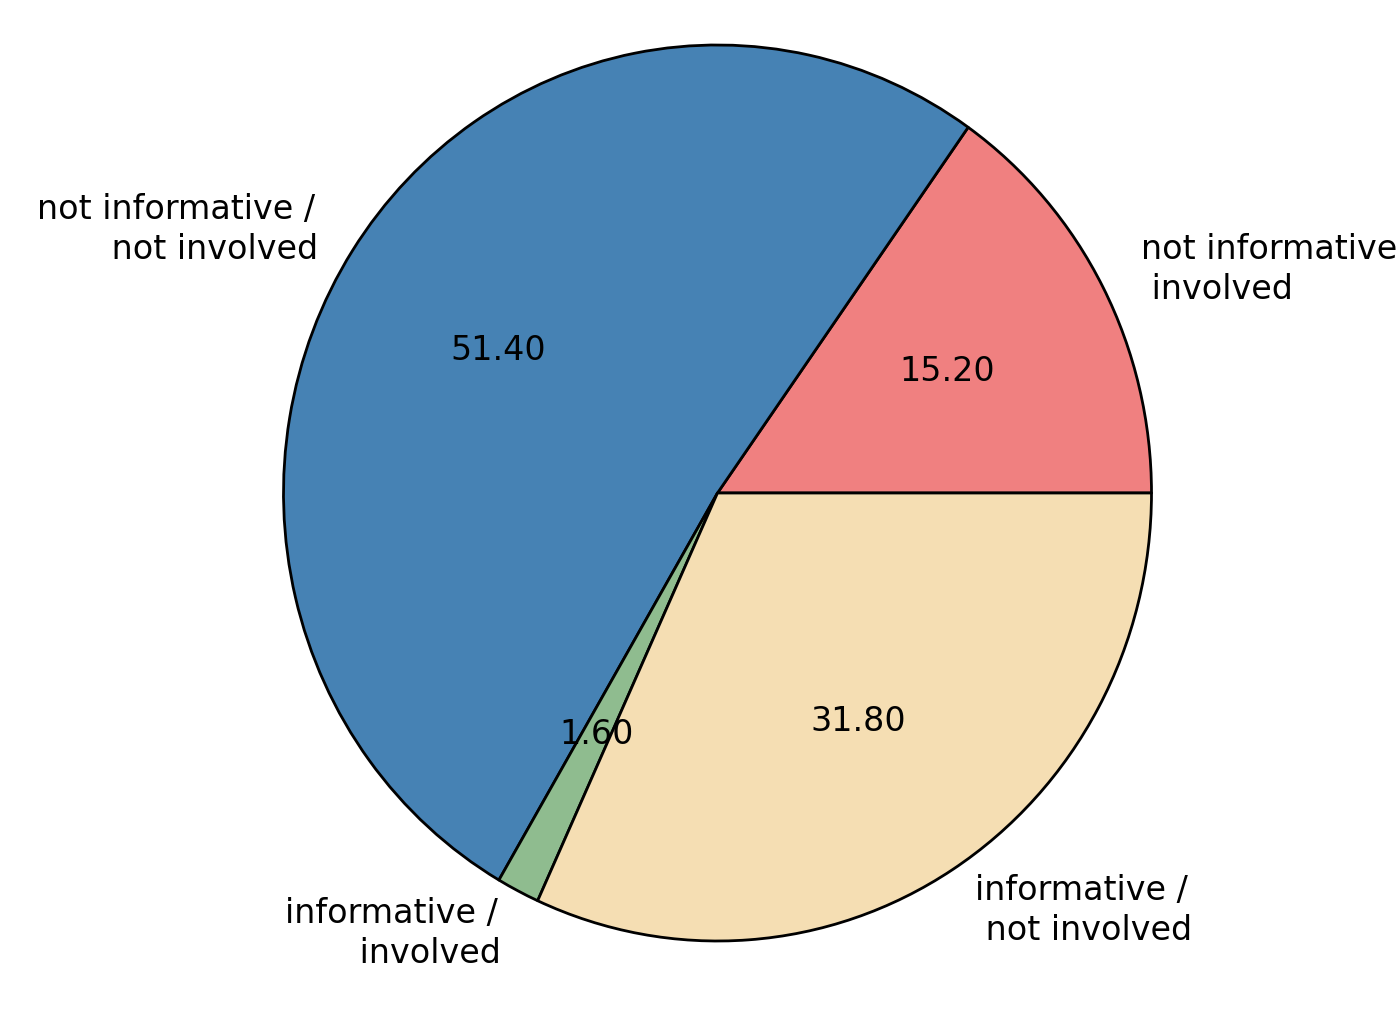
\includegraphics[width=0.5\textwidth]{images/plots/pies/pie_pairs.png}
\caption{Tweets type repartition for the informative and involved features}
\label{pieTypeInfInv}
\end{figure}
\begin{figure}[H]
\centering
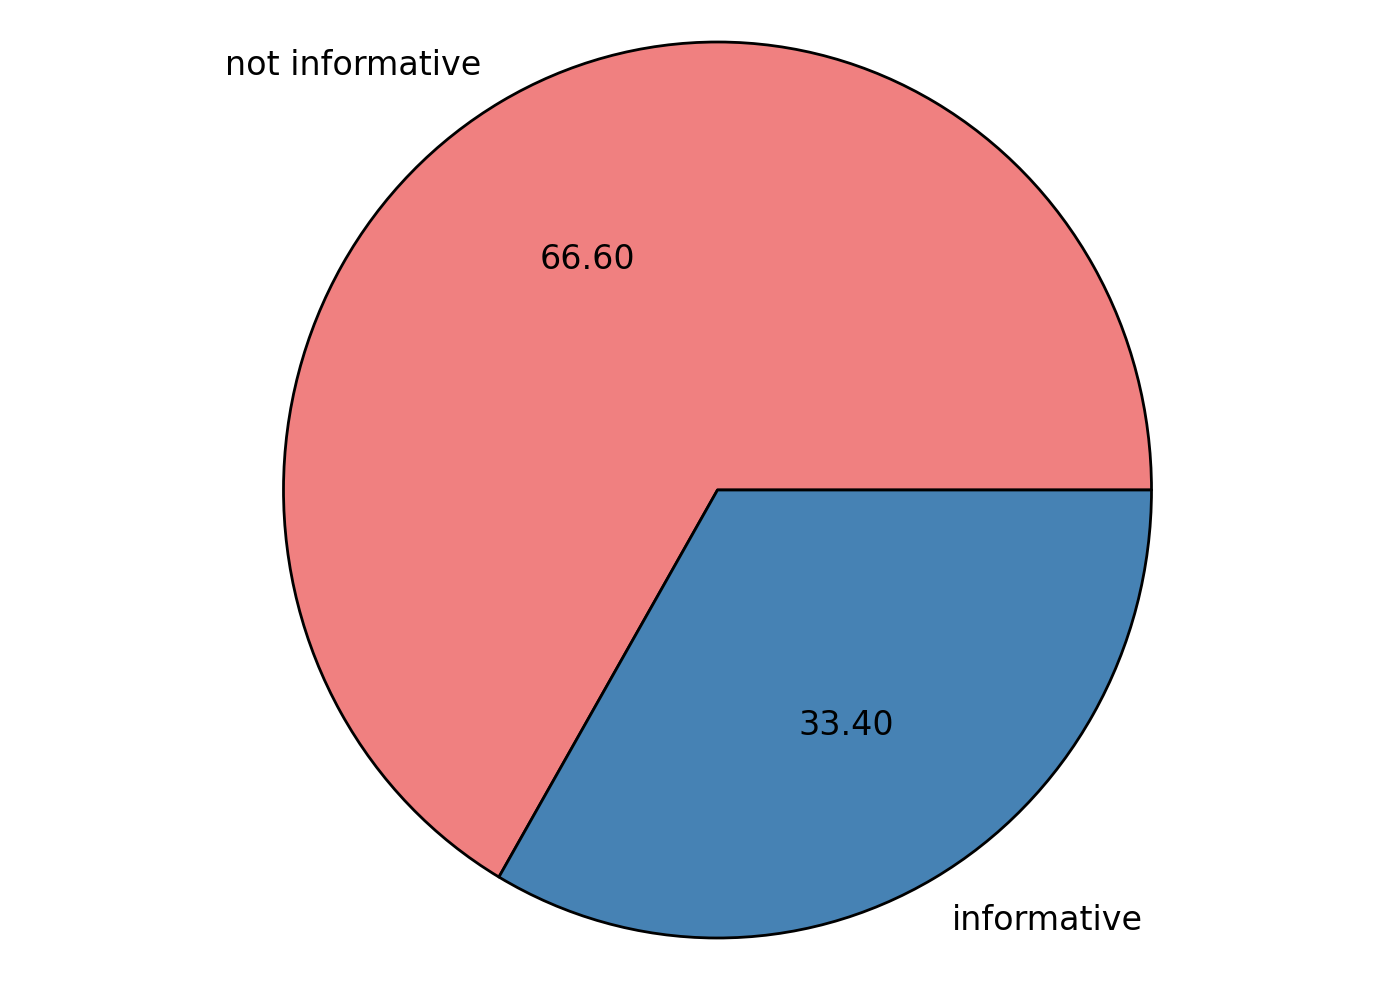
\includegraphics[width=0.5\textwidth]{images/plots/pies/pie_info.png}
\caption{Tweets type repartition for the informative feature}
\label{pieTypeInf}
\end{figure}
\begin{figure}[H]
\centering
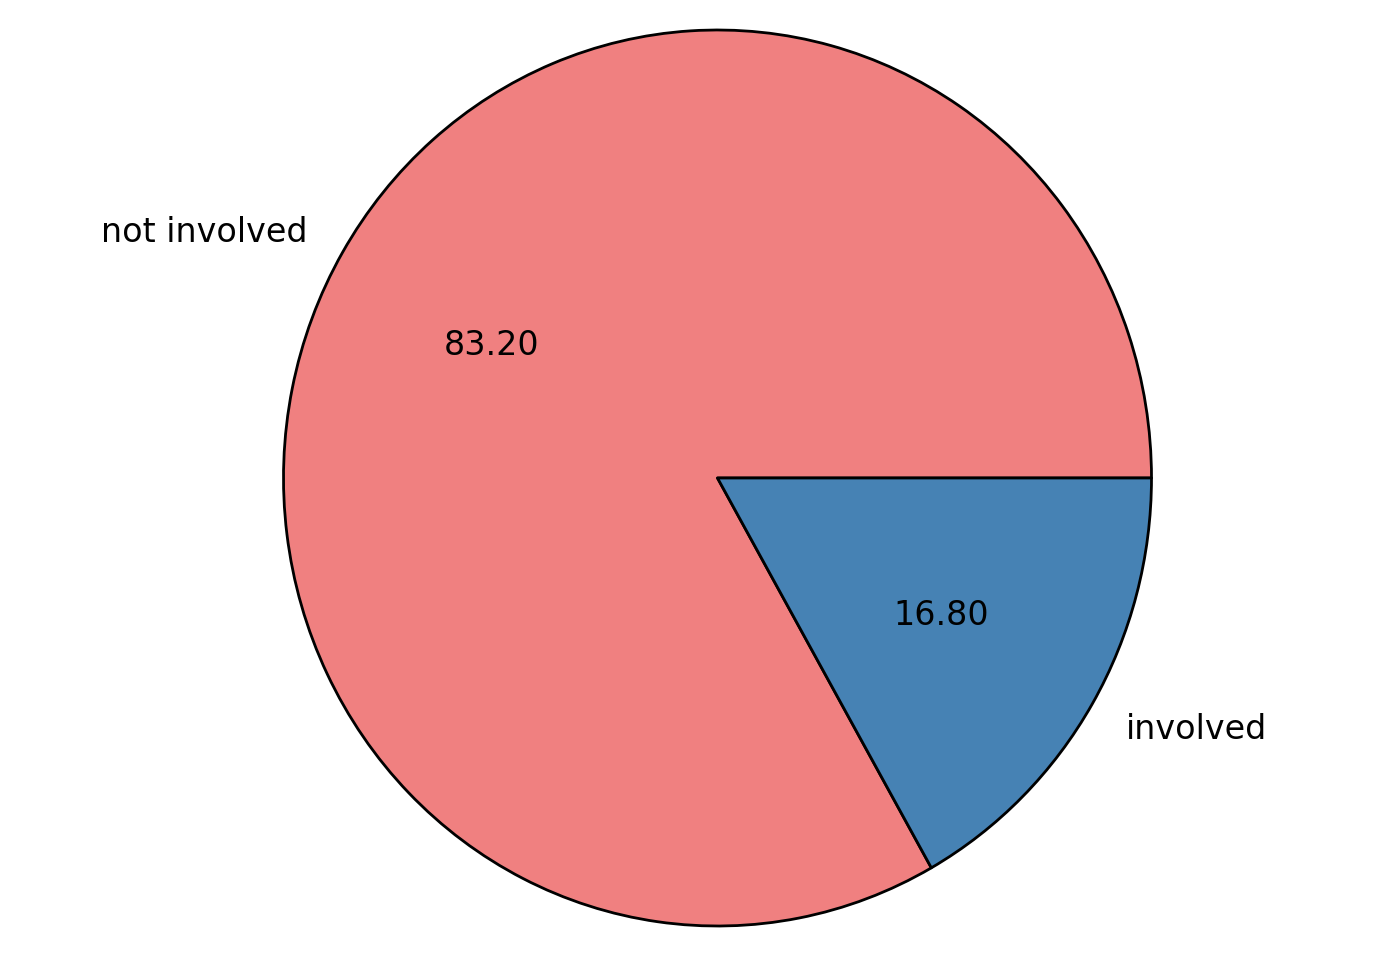
\includegraphics[width=0.5\textwidth]{images/plots/pies/pie_invo.png}
\caption{Tweets type repartition for the involvement feature}
\label{pieTypeInv}
\end{figure}
\vspace*{-0.6cm}
\begin{figure}[H]
\centering
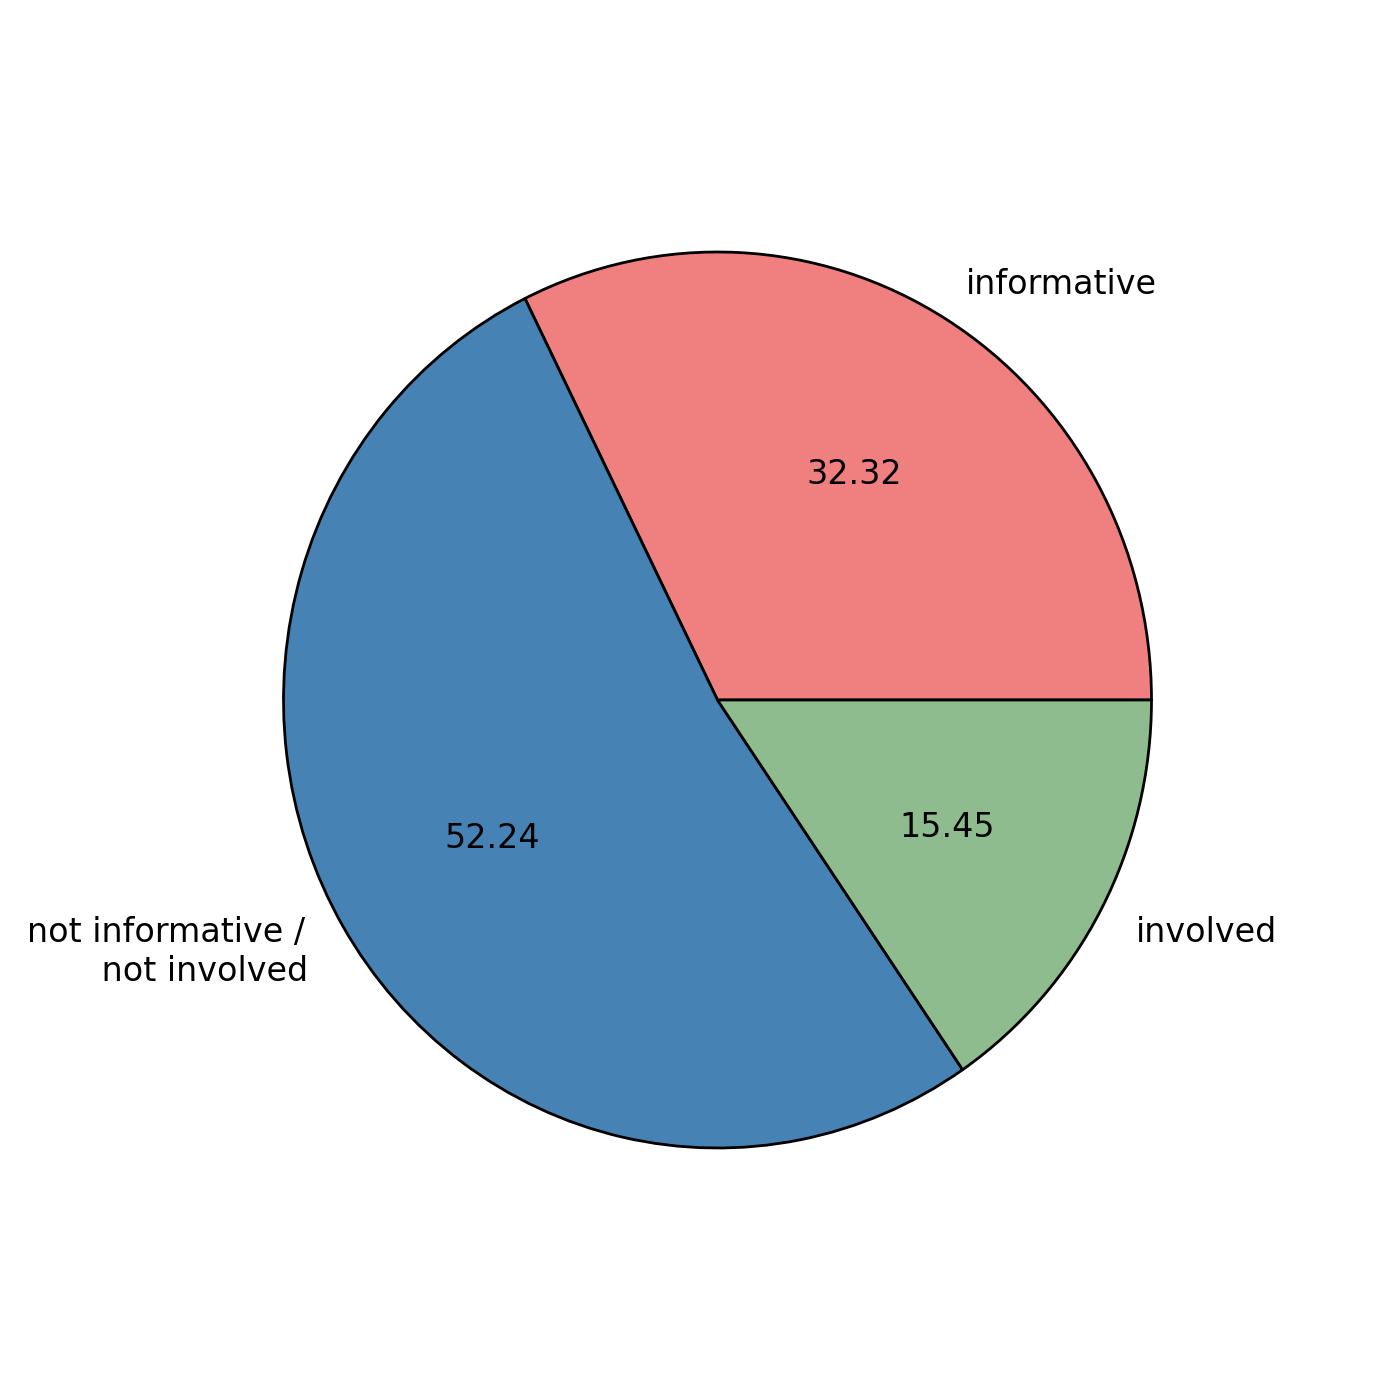
\includegraphics[width=0.46\textwidth]{images/plots/pies/pie_pairs3.png}
\caption{Proportions in dataset}
\end{figure}

To visualize the repartition of the features informative and involvement, we plot the following pies.\\
Firstly, one can notice on the figure \ref{pieTypeInfInv} how the types are divided : 
\begin{itemize}
\item half of the tweets are neither informative nor involved. This is what we can call the \emph{garbage} category, as the concerned tweets are not worthy of interest.
\item a very small part ($\sim$ 1.6\%) is both informative and involved. Considering the small percentage, we can consider this category is not significant.
\item the remaining are either (exclusively) involved or informative, with almost 2 times more informative tweets.
\end{itemize}

The figures \ref{pieTypeInf} and \ref{pieTypeInv} show the type repartition only for respectively the informative and involvement features, and lead to the following statements :
\begin{itemize}
\item more that half ($\sim$ 67\%) of the tweets contain no informative content.
\item surprisingly, only a bit more than a quarter ($\sim$ 17\%) are involved.
\end{itemize}


\end{multicols}

\subsubsection{Testing}
In order to test the model accuracy, we use the $k$-fold cross-validation technique with the $F_1$-score.

The easiest way to test a model is to split a labeled dataset in two parts : the training set $s_1$ (for example 80\% of the whole dataset) and the testing set $s_2$ (20\%). Once the model is trained with the set $s_1$, we run the model with the test set $s_2$, and compare the predicted labels with the true labels of $s_2$.

For a better trusted accuracy, it is common to use \textbf{$k$-fold cross-validation} method :
\begin{enumerate}
\item divide the dataset in $k$ parts ;
\item use the first part as the testing set, and the union of the $k-1$ other parts as the training set ;
\item compute accuracy (in our case the $F_1$-score) ;
\item rotate such as each part is used once as the testing set and the others as training set ;
\item compute the average accuracy
\end{enumerate}

For the accuracy, we use the $F_1$-score, given by :
$$ F_1  = \frac{2\cdot\text{true positive}}{2\cdot\text{true positive}+\text{false negative}+\text{false positive}} $$

The test results are shown in figure \ref{nb1testresults}, with $k$ = 5. NB refers to Multinomial Naive Bayes, and PNB to Pair Multinomial Naive Bayes, as described before. We try to train the model with unigrams (tokens of single words) and bigrams (tokens of two words). The best result are obtained with unigrams with the NB model, as achieve a average accuracy of almost 65\%. However, the score of class 2 remains bad (14.5\%), so the model does not currently suit to classify our tweets. Two reasons appear :
\begin{enumerate}
\item it is harder to characterize class 2 by its content than the other classes ;
\item we do not have enough data to train the model.
\end{enumerate}

\begin{figure}[H]
  \centering
\begin{tabular}{c|c|c|c|c||||c|}
\cline{2-6}
& class \# & 0 & 1 & 2 & \multirow{2}{*}{average}\\ \cline{2-5}
% & proportion & 52\% & 32\% & 15\%  & \\ \cline{2-5}
& meaning & $\neg$ if $\&$ $\neg$ iv & if $\&$ $\neg$ iv & $\neg$ if $\&$ iv  & \\
\hline
\multicolumn{1}{|c|}{\multirow{2}{*}{\rotatebox{90}{NB}}} & unigrams & 76.1\% & 72.8\% & 14.5\% & 64.9\% \\
\multicolumn{1}{|c|}{} & bigrams & 74.3\% & 68.4\% & 4.2\% & 61.1\%   \\
\hline
\hline
\multicolumn{1}{|c|}{\multirow{2}{*}{\rotatebox{90}{PNB}}} & unigrams & 68.6\% & 70.0\% & 18.9\% & 60.8\% \\
\multicolumn{1}{|c|}{} & bigrams & 62.5\% & 64.5\% & 10.1\% & 54.6\%   \\
\hline
\end{tabular}
\caption{Accuracies 5-fold cross-validation ; if = informative, iv = involved}
\label{nb1testresults}
\end{figure}

\newpage

\section{Media analysis}
As seen in the previous part, it is difficult to classifiy the biased tweets only by the language.

\subsection{Motivation}
One can notice on figure \ref{mediaFreq11} that the tweets containing a media represent half of the total tweets, on average. As a result, it is important to take it into consideration and analyze it.

\begin{figure}[H]
\centering
\includegraphics[width=0.5\textwidth]{images/freqs/medias/freq_meds_11.png}
\caption{Medias proportion on August 11th}
\label{mediaFreq11}
\end{figure}

If we take a look at the tweets on the 11th of August labeled as biased, we can extract the medias on the figure \ref{tweets500mediasBiaised}. On the left, there is the domain names of the medias and on the right their descriptions.

The medias types are various : videos, images, blog articles, chatting window etc.
\begin{figure}[H]
  \centering
\begin{tabular}{|c|c|}
\hline
media domain name & description \\ \hline
\texttt{youtube.com} & Anonymous Operation video \\ \hline
\texttt{cnn.com} & video of Brown's mother ``you took my son away from me" \\ \hline
\texttt{vine.co} & a man encouraging the protesters. ``No fear. Keep going." \\ \hline
\texttt{twimg.com} & picture about racism \\ \hline
\texttt{talk.ee} & chat window \\ \hline
\texttt{theobamacrat.com} & blog article defending Mike Brown \\ \hline
\texttt{twitter.com} & tweet/photo of an activist (deleted since) \\ \hline
\texttt{stltoday} & article defending Mike Brown \\ \hline
\texttt{youtube.com} & video clip encouraging riots \\ \hline
\hline
\end{tabular}
\caption{Medias in the training set labeled as supportive}
\label{tweets500mediasBiaised}
\end{figure}

\newpage

\subsection{Formulation}
Let's define $ \mathcal{M}_r = \{ m \} $ the set of medias $m$ shared during the riot $r$. Each media is associated to $n$ different tweet messages, without considering retweets.

\textbf{Hypothesis :} if the class of a media $m$ is $C \in \{0,1,2\}$ then the associated tweet messages belongs also to this class.

\subsection{Annoting the top 100 medias}
\label{annotingTopMediasSection}

We first consider the 100 medias the most retweeted on the 11th of the August, and we label it manually :
\begin{itemize}
\item \textbf{garbage} (class 0)
\item \textbf{informative} (class 1)
\item \textbf{biased} (class 2)
\end{itemize}

\begin{figure}[H]
\begin{minipage}[t]{0.45\textwidth}
\begin{center}
	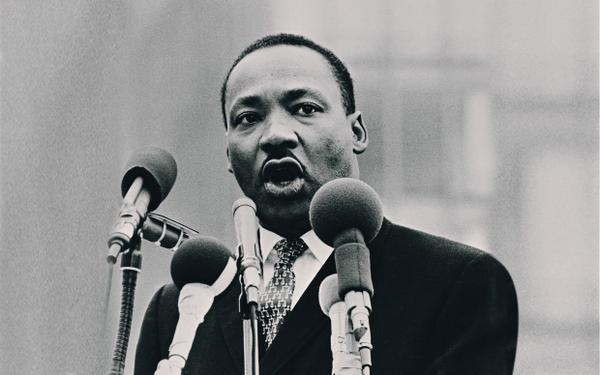
\includegraphics[width=\textwidth]{images/photos/mlk.jpg}
	\caption{Media the most shared on the 11/08 night}
\end{center}
\end{minipage}
\hfill
\begin{minipage}[t]{0.4\textwidth}
\begin{center}
	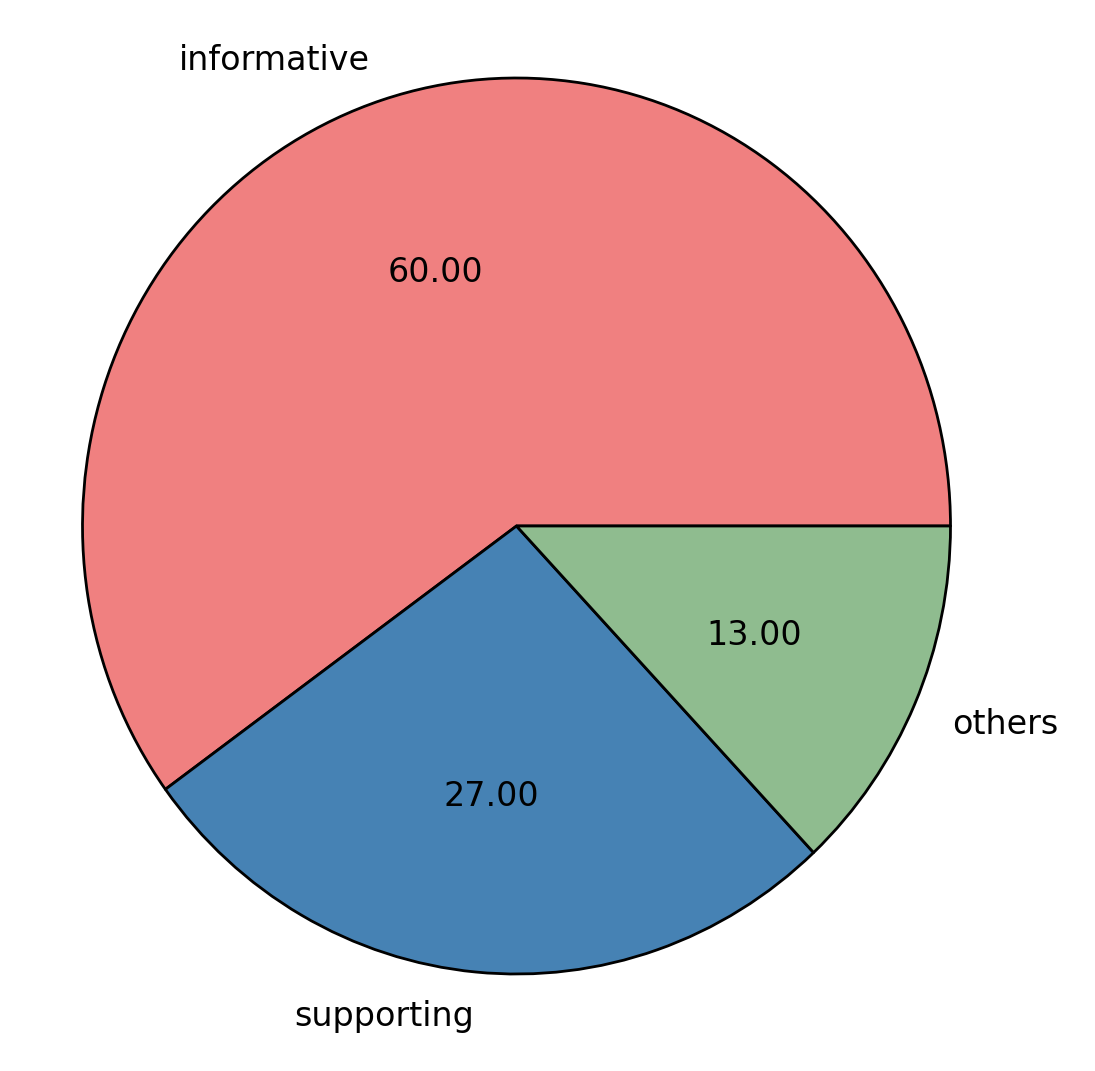
\includegraphics[width=\textwidth]{images/plots/pies/pie_medias.png}
	\caption{Media type repartition on the 11/08}
	\label{typeRepartitionMedias}
\end{center}
\end{minipage}
\end{figure}

The type repartition can be seen on the figure \ref{typeRepartitionMedias}

\newpage

\subsection{Improving the classification model}
\label{NBMediaSec}

Annoting only 100 medias enables to actually label several thousand tweets.
\begin{figure}[H]
  \centering
\begin{tabular}{c|c|c|c|c||||c|}
\cline{2-6}
& class \# & 0 & 1 & 2 & \multirow{2}{*}{average}\\ \cline{2-5}
& meaning & $\neg$ if $\&$ $\neg$ iv & if $\&$ $\neg$ iv & $\neg$ if $\&$ iv  & \\
\hline
\multicolumn{1}{|c|}{\multirow{2}{*}{\rotatebox{90}{NB}} } & unigrams & 84.9\% & 97.4\% & 85.9\% & 95.3\% \\
\multicolumn{1}{|c|}{} & bigrams & 80.4\% & 97.4\% & 78.5\% & 94.7\%   \\
\hline
\hline
\multicolumn{1}{|c|}{\multirow{2}{*}{\rotatebox{90}{PNB}}} & unigrams & 85.9\% & 97.6\% & 85.7\% & 95.6\%   \\
\multicolumn{1}{|c|}{} & bigrams & 83.2\% & 97.5\% & 79.9\% & 95.1\%   \\
\hline
\end{tabular}
\caption{Accuracies 5-fold cross-validation ; if = informative, iv = involved}
\end{figure}

Given one of our Naive Bayes model, it is easy to get the most informative features of each class. These are shown on figures \ref{impfeatureclass1} and \ref{impfeatureclass2}.

\begin{figure}[H]
\begin{minipage}[t]{0.5\textwidth}
\begin{center}
	\includegraphics[width=\textwidth]{images/diags/media_features_1.png}
	\caption{Most important features of the class 1}
	\label{impfeatureclass1}
\end{center}
\end{minipage}
\hfill
\begin{minipage}[t]{0.42\textwidth}
\begin{center}
	\includegraphics[width=\textwidth]{images/diags/media_features_2.png}
	\caption{Most important features of the class 2}
	\label{impfeatureclass2}
\end{center}
\end{minipage}
\end{figure}

One can see how the features of class 1 gather descriptive words, such as \emph{looting}, \emph{burning}, \emph{shots} etc. The class 2 talks about the \emph{hackers} and use different kind of words.

\newpage
\subsection{Media embedding and visualization}

In this section we try to visualize the users given the medias they published.\\
In order to achieve this, we represent a user by a media vector, in the same way we did in section \ref{tweetEmbeddingSection} but now with medias.

\[
\bordermatrix{~ & media_1 & media_2 & \cdots & media_n \cr user_1 =  & tfidf_{1,1} & tfidf_{1,2} & \cdots & tfidf_{1,n} \cr}
\]

Given the $n$ most shared medias during a riot, each component $i$ of the vector is the $tfidf$ frequency of the media $i$ for the user.

Moreover, if the users posted a media that appears in the top 100 medias we labeled (section \ref{tweetEmbeddingSection}) as classified as \emph{supportive}, we mark the user as ``supportive".

Eventually, we take the 1000 most active users, apply $t$-SNE transformation and plot it, as shown on figure \label{tsneMedias}. The black dots represent the ``supportive" users, and the grey dots the others. One can notice on the figure \label{tsneMedias} that two clusters appear.

\begin{figure}[H]
\centering
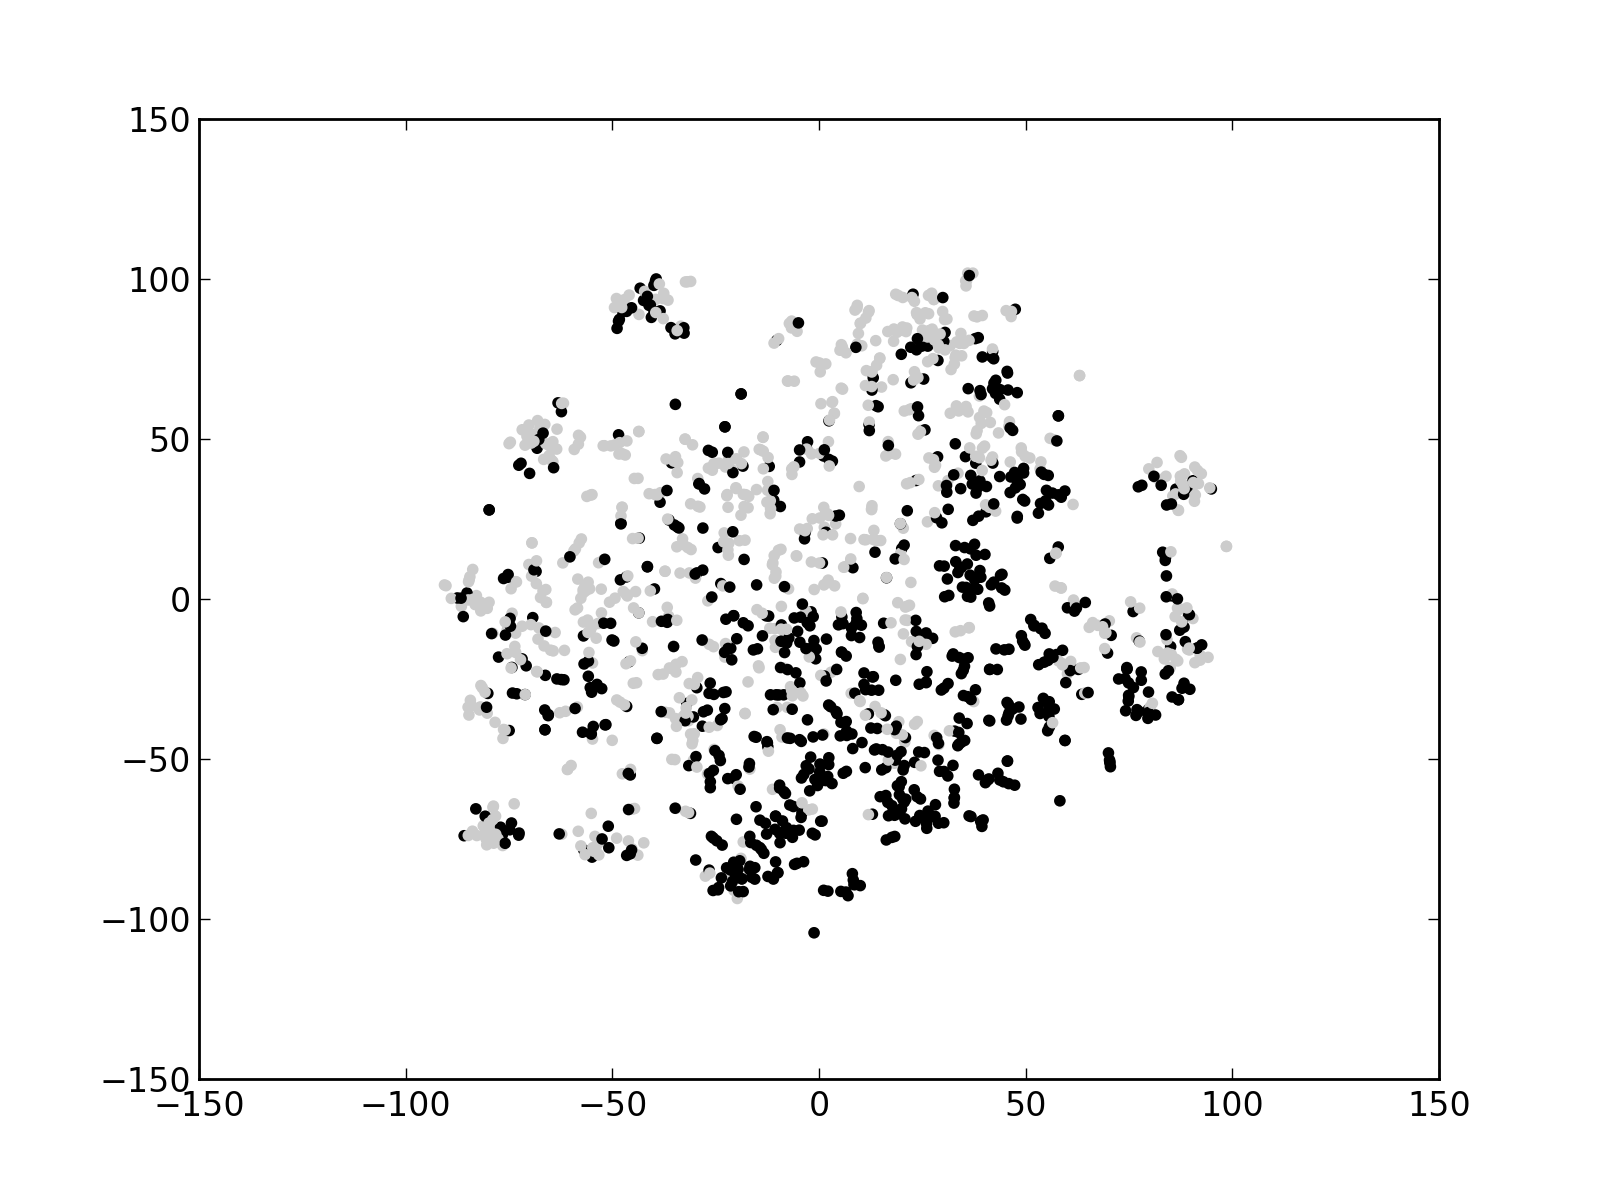
\includegraphics[width=\textwidth]{images/plots/media_tsne.png}
\caption{$t$-SNE transformation applied on the media vectors}
\label{tsneMedias}
\end{figure}


%%%%%%%%%%%%%%%%%%%%%%%%%%%%%%%%%%%%%%%%%%%%%%%%%%%%%%%%%%%%%%%%%%%%%%%
%%%%%%%%%%%%%%%%%%%%%%%%%%%%%%%%%%%%%%%%%%%%%%%%%%%%%%%%%%%%%%%%%%%%%%%
%%%%%% CHAPTER 5 - INFLUENCE NETWORK
%%%%%%%%%%%%%%%%%%%%%%%%%%%%%%%%%%%%%%%%%%%%%%%%%%%%%%%%%%%%%%%%%%%%%%%
%%%%%%%%%%%%%%%%%%%%%%%%%%%%%%%%%%%%%%%%%%%%%%%%%%%%%%%%%%%%%%%%%%%%%%%

\chapter{Graph analysis and influence network}

\section{Motivation and outline}

In the past chapters we focused on the content analysis of the tweets. However, we have to keep in mind that we are working with data from a social network. As a consequence, it is important to study the underlying graphs interesting for our objectives.

In this chapter we start with computing several graphs in order to explore the dataset, then, we will focus on how to define influence in a network.

\newpage
\section{Hashtags graph}
We start with analyzing the hashtags combinations. We construct a undirected graph such as :
\begin{itemize}
\item a \textbf{node} represents a hashtag
\item an \textbf{edge} between nodes $a$ and $b$ exists if $a$ and $b$ are used together is a tweet. Our edges are weighted such as the higher the weight, the more used hashtag combinaison.
\end{itemize}

\subsection{Computation}

The algorithm \ref{algo:hashtagsGraph} builds a graph of the hashtags combinaisons.

\begin{algorithm}
\caption{Create hashtags graph}
\label{algo:hashtagsGraph}
\begin{algorithmic} 
\STATE \textbf{input} : tweets list, empty graph
\STATE \textbf{output} : graph
\FOR{each tweet in list}
\FOR{each hashtag}
	\STATE add hashtag to list
	\IF{node 'hashtag' does not exist in graph}
	\STATE add hashtag node to graph
	\ENDIF
	\FOR{each couple in 2-permutations of list elements}
	\IF{edge 'couple' does not exist in graph}
	\STATE add couple edge to graph
	\ELSE
	\STATE increase weight of the couple edge in graph
	\ENDIF
	\ENDFOR
\ENDFOR   
\ENDFOR
\\[10pt]
\hspace{-22pt}
\greybox{$\rhd$ \textbf{\underline{Complexity}}: 
The number of hashtags in a tweet is low (en general below 5 and often 0). Thus, for the time complexity we only consider the first for loop, which gives us a \textbf{$\mathcal{O}(n)$} time complexity.
}
\end{algorithmic}
\end{algorithm}

One can see the result on figure \ref{graphHt13nc}. On this graph, only the top 100 edges are shown, and the hashtag \texttt{\#ferguson} as been removed, considered as trivial. The more visible the edge, the higher the weight.


// redo graph

\begin{figure}[H]
\centering
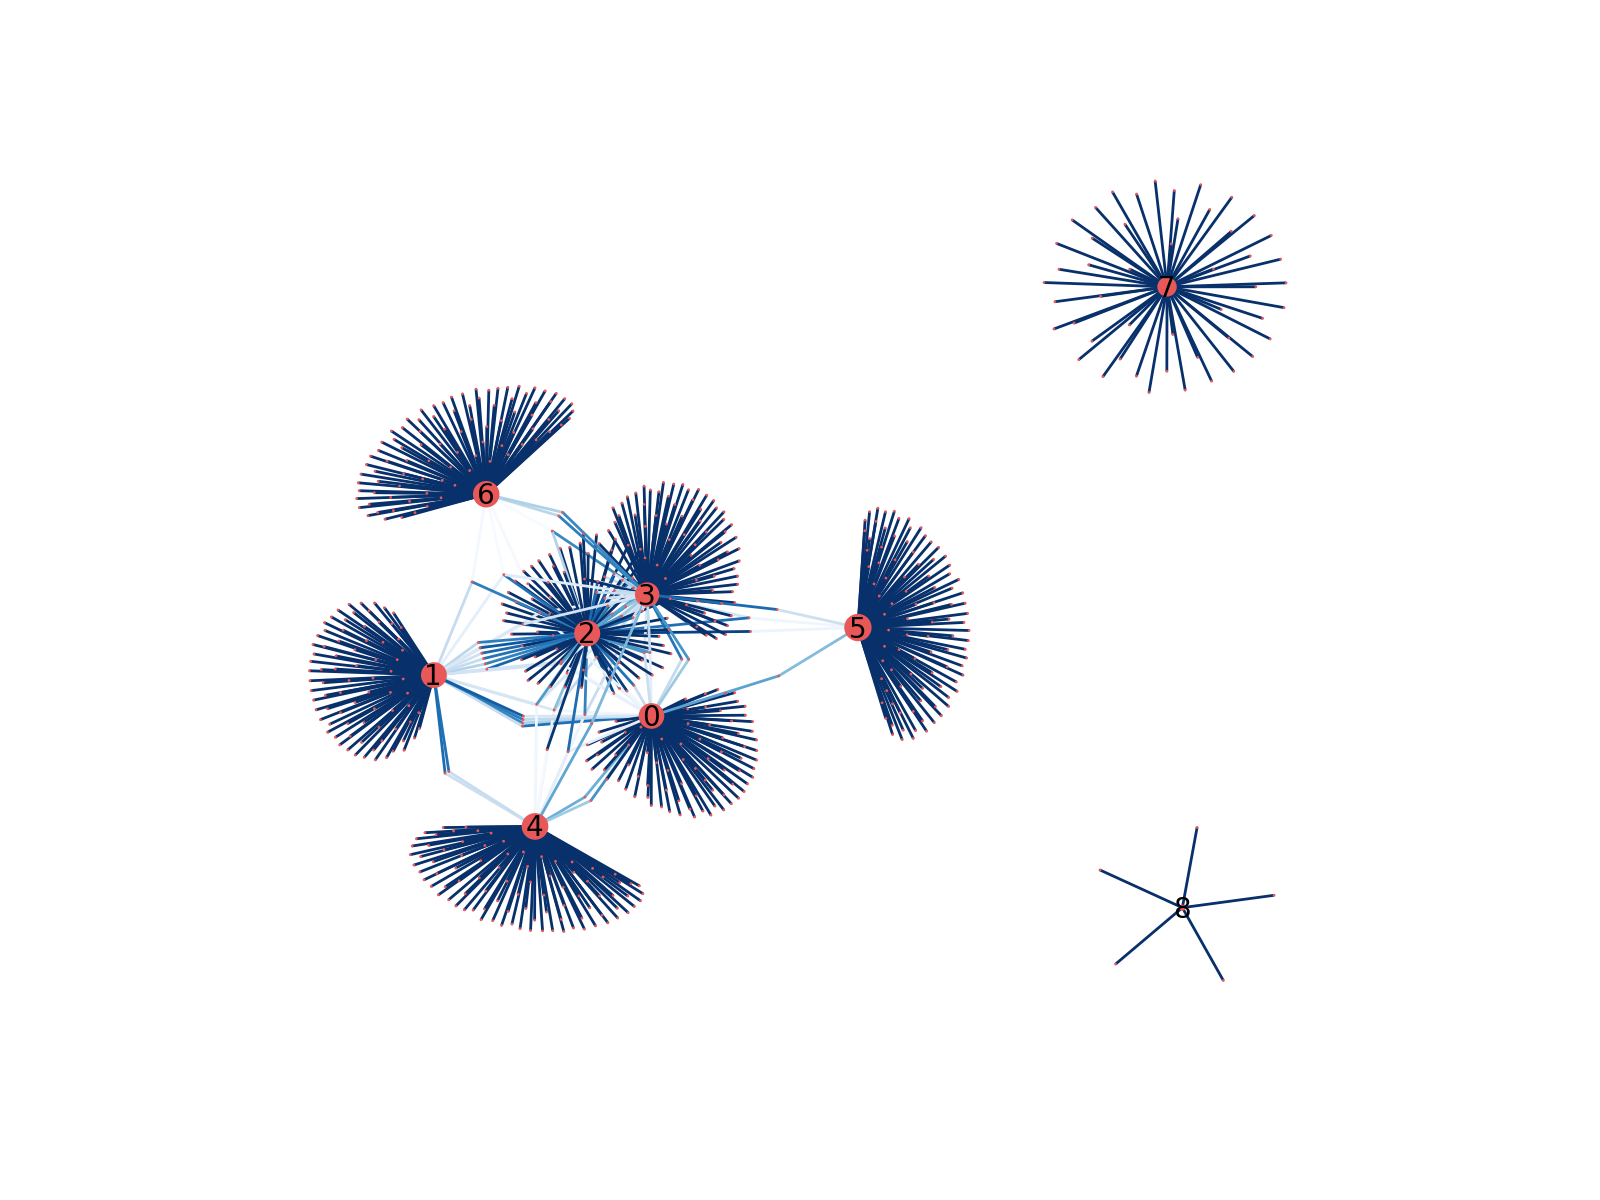
\includegraphics[width=\textwidth]{images/graphs/hashtags/13_08.png}
\caption{Hashtag graph for the August 13th.}
\label{graphHt13nc}
\end{figure}

\subsection{Community detection}
On the figure \ref{graphHt13nc}, there are evident groups of hashtags that can be considered as \emph{communities}. In this section we try to detect automatically such communities in the graph.

In order to achieve this, we use the algorithm described in \cite{blondel2008fast}, based on graph modularity optimization, and implemented in python by T. Aynaud\footnote{http://perso.crans.org/aynaud/communities/}.

The modularity\cite{newman2006modularity} of a group can be defined as the observed number of edges in that group minus the expected number of edges if they were distributed randomly.

The number of communities to detect is a parameter of the algorithm. In our case, we set this parameter equals to 5.

The obtained graph is shown on figure \ref{graphHt13c}.

\vfill

\begin{figure}[H]
\centering
\includegraphics[width=\textwidth]{images/graphs/hashtags/hc_13_08.png}
\caption{Hashtag graph}
\label{graphHt13c}
\end{figure}

One can notice on the figure \ref{graphHt13c} we obtain distinct communities with different contents :

\definecolor{c_purple}{HTML}{862B59}
\definecolor{c_red}{HTML}{A10000}
\definecolor{c_green}{HTML}{0A6308}
\definecolor{c_blue}{HTML}{123677}
\definecolor{c_orange}{HTML}{FF8100}

\begin{itemize}
\item \textbf{\textcolor{c_purple}{community \#1}} : political content related to the conservatives christians (\texttt{\#ccot}), the conservatives, the democratic party (\texttt{\#dem}), the republican party (\texttt{\#gop}) etc.
\item \textbf{\textcolor{c_red}{community \#2}} : general content about black activist (Cornel W. Brooks), a friend of Mike Brown (Dorian Johnson), corruption etc.
\item \textbf{\textcolor{c_green}{community \#3}} and \textbf{\textcolor{c_blue}{community \#4}}: close communities with similar content related to defense of the blacks, with expressions like ``black lives matter", ``black youth matter", ``hands up don't shoot", ``dont't shoot" etc.
\item \textbf{\textcolor{c_orange}{community \#5}} : content relative to the Middle East, like Afghanistan, Baghdad and Israel (\texttt{\#bds}).
\end{itemize}

\newpage
\subsection{Contribution graph}

We can wonder how users actually contribute to these hashtags communities. Do users frequently tweet with hastags of a same community or tweet in several hashtags communities ? For this purpose, we take the 100 users who tweeted the most in a community and we see if they tweeted in others communities. A big red dot represent a community with a given number, a small dot represent a user. A edge, in blue, links a user and a community. The opacity of the edge represents the proportion of the users tweets. The more the edge is dark blue, the more the user contributed to that community. The result is shown on figure \ref{contribGraph}.

\begin{figure}[H]
\centering
\includegraphics[width=\textwidth]{images/graphs/hashtags/contrib_13_08.png}
\caption{Hashtag graph}
\label{contribGraph}
\end{figure}

One can clearly see that most of the users only contributed in only one community. As a consequence, this means that hashtags induce both content and users communities.

\newpage

\section{Retweets graph}
The other graph we can easily compute from our dataset is the mentions graph. As studied in section \ref{subSecFreqs}, a large proportion of tweets are retweets. As a consequence, we decide to keep only the retweet mentions in the graph, such as :
\begin{itemize}
\item a \textbf{node} represents a user
\item an \textbf{directed edge} from node $a$ to $b$ exists if $a$ retweets $b$. Our edges are weighted such as the higher the weight is, the more $a$ has retweeted $b$.
\end{itemize}

\subsection{Computation}

The algorithm \ref{algo:rtGraph} builds a graph of the retweets.

\begin{algorithm}
\caption{Create retweets graph}
\label{algo:rtGraph}
\begin{algorithmic} 
\STATE \textbf{input} : retweets list, empty graph
\STATE \textbf{output} : graph
\FOR{each retweet in list}
	\STATE // we call $a$ the the retweet author
	\STATE // and $b$ the author of the original tweet
	\IF{nodes $a$ does not exist in graph}
	\STATE add hashtag node $a$
	\ENDIF
	\IF{nodes $b$ does not exist in graph}
	\STATE add hashtag node $b$
	\ENDIF
	\IF{edge $a \rightarrow b$ does not exist in graph}
	\STATE create edge $a \rightarrow b$
	\ELSE
	\STATE increase weight of edge $a \rightarrow b$
	\ENDIF
\ENDFOR
\FOR{each node in graph}
	\STATE keep the most important outgoing edge
\ENDFOR
\end{algorithmic}
\end{algorithm}

The result for the August 17th is shown on figure \ref{rtGraph17}.

\begin{figure}[H]
\centering
\includegraphics[width=\textwidth]{images/graphs/rtmentions/rtmentions_17.png}
\caption{Retweet graph for the August 17th}
\label{rtGraph17}
\end{figure}

On figure \ref{rtGraph17}, we can clearly see the users that have been retweeted a lot : these are the big mass of points (the edges are not visible as they are too many points).

Moreover, the graph does not contain only one group but several, and these groups are connected each other. We obtain a \emph{star} disposition, espacially on the left, as small groups are connected to a big group.

This graph highlights the influence in the network. In big groups there are underlying very influent nodes. We can then say that the two big groups  in the center of the graph represent the most influent users. In the same way, the nodes at the end are not influent in the network.

As a result, the aim is now to measure this influence, that is to say, that kind of position in the graph. We broach this point in the next section.

\newpage
\section{Influence in graph}	
\subsection{Defining the influence}

\subsubsection{Degree Centrality}
The degree centrality is the most simple way to characterize the influence of a node in a network. It is simply depends on the number of edges connected to the node. The more a node has edges, the more it is important in the network.

The degree centrality of node $i$ is given by :

$$ C_d(i) = \frac{d(i)}{n-1} $$

where d(i) is the degree of the node $i$ and $n$ is the number of nodes in the graph.

However, this measure has limits. Indeed, the node degree is local measure and it does not take into consideration the whole network structure.

\subsubsection{Page Rank}
\label{PRSec}
The Page Rank\cite{page1999pagerank} was originally designed for web pages but it can be used for any kind of graph.

The main idea of the Page Rank is that an important node is pointed by other important nodes.

The Page Rank PR of a node $i$ is given by :

$$ PR(i) = \alpha \sum_{j \rightarrow i} \frac{PR(j)}{\textsf{out}(j)} + \frac{1-\alpha}{n} $$

where :
\begin{itemize}
\item $\textsf{out}(j)$ is the outdegree of $j$
\item $n$ is the number of nodes in the graph
\item $\alpha$ is the \emph{damping factor}, a constant parameter
\end{itemize}

We make an experiment with these two measures in the following part.

\newpage

\subsection{Experiment}

We compute both In-degree centrality and Page Rank on the August 17th graph and we compare the top influent users lists obtained from these two measures. The result is shown on figure \ref{topinfluentTab11}. The corresponding graph is shown on figure \ref{gi17}.

\vspace{1cm}

\begin{figure}[H]
  \centering
\begin{tabular}{ccc}
\hline
Rank & \textbf{In-Degree Centrality} & \textbf{Page Rank}\\ \hline \hline
1 & ryanjreilly & ryanjreilly \\ \hline
2 & antoniofrench & \cellcolor{red!20} huffingtonpost \\ \hline
3 & youranonnews & youranonnews \\ \hline
4 & fergusonunity & antoniofrench \\ \hline
5 & youranonglobal & fergusonunity \\ \hline
\hline
\end{tabular}
\caption{Top influent users on the August 17th}
\label{topinfluentTab11}
\end{figure}

\vspace{1cm}

\begin{figure}[H]
\centering
\includegraphics[width=\textwidth]{images/graphs/influence/gi_t0_1708.png}
\caption{Influence graph on the August 17th}
\label{gi17}
\end{figure}

\newpage

We can notice the \texttt{huffingtonpost} node does not appear in the top influent nodes with the degree centraliy measure. Indeed, it has a small degree but an incoming edge from the node \texttt{ryanjreilly}, so \texttt{huffingtonpost} is an influent node and only detected by the Page Rank measure.

The polarity is given by the green (= supportive) / yellow (= informative) colorbar. The top 10 influent users (given by Page Rank) are named on the graph. If a name is in dark, the corresponding user has a negative polarity. If a name is in light, the user has a positive (or null) polarity. 

Firstly, one can notice 


\chapter{Role of a user}

\section{Definition}
In this chapter we define and represent the role of a user during one or several riots based on the previous work. In the chapters 4 and 5, we introduced the \emph{polarity} and \emph{influence} scores for a user for a given set of tweets. Given the topics for a considered riot obtained in chapter 3, we can define :
\begin{itemize}
\item the \emph{polarity vector} of a user for a riot as being the vector of the polarities of this user computed for the different topics belonging to the considered riot ;
\item the \emph{influence vector} of a user for a riot as being the vector of the influences of this user computed for the different topics belonging to the considered riot ;
\end{itemize}
We can now define the role of a user in a riot as follow : 

\begin{defbox}
\textbf{Definition} - Role of a user for a riot \\[10pt]
Let $u$ be a user and $r$ a riot with $n$ topics. \\
Given the polarity vector $ \mathcal{P}(u) = (p_{t_1},p_{t_2},\cdots,p_{t_n}) $\\ \hspace*{20pt} where $(p_{t_i})_{1\leq i\leq n}$ is the polarity of $u$ for the topic $t_i$,\\
And given the influence vector $ \mathcal{I}(u) = (i_{t_1},i_{t_2},\cdots,i_{t_n}) $\\ \hspace*{20pt} where $(i_{t_i})_{1\leq i\leq n}$ is the polarity of $u$ for the topic $t_i$,\\[10pt]
We can define the \emph{role} $ \mathcal{R}(u) $ of $u$ as being the concatenation of $\mathcal{P}(u)$ and $\mathcal{I}(u) : $
$$ \mathcal{R}(u) = (\mathcal{P}(u) | \mathcal{I}(u)) $$
\end{defbox}

\newpage

In a similar way, we can easily define the role of a user for $m$ riots by concatenation : 

\begin{defbox}
\textbf{Definition} - Role of a user for $m$ riots \\[10pt]
Let $u$ be a user and let $s = \{r_i\}_{1\leq i\leq m}$ a set of $m$ riots with $n$ topics each. \\
Given the polarity vector $ \mathcal{P}_{r_i}(u) = (p_{t_1},p_{t_2},\cdots,p_{t_n}) $ of $u$ for the riot $r$ and in the same way $ \mathcal{I}_r(u) = (i_{t_1},i_{t_2},\cdots,i_{t_n}) $ its influence vector, we can define the new polarity and influence vectors for $u$ for the set $s$ as follow : 
$$ \mathcal{\hat{P}}(u) = (\mathcal{P}_{r_1}|\mathcal{P}_{r_2}|\cdots|\mathcal{P}_{r_m}) $$
$$ \mathcal{\hat{I}}(u) = (\mathcal{I}_{r_1}|\mathcal{I}_{r_2}|\cdots|\mathcal{I}_{r_m}) $$
and the role of $u$ for $s$ as : 
$$ \mathcal{\hat{R}}(u) = (\mathcal{\hat{P}}(u) | \mathcal{\hat{I}}(u)) $$
\end{defbox}

\section{Dimension reduction}
\label{dimReducSection}

\subsection{High-dimensional vectors}
The vectorial space created is currently 10 dimensional. This can be considered as high-dimensional and as a consequence causing trouble. 

Firstly, because of the \textbf{curse of dimensionality}. In high dimensions, the space is big and sparse. As a consequence, it becomes difficult to evaluate if two vectors are similar/close or not.

Secondly, it is interesting to reduce the dimensions for \textbf{visualization} purpose.

\subsection{Principal Component Analysis}
Principal Component Analysis is a well-known statistical method to reduce dimensions of a dataset. It converts a set of correlated components to a new set of uncorrelated ones called principal components.

Each principal components explain a percentage of variance such as the first components have the highest variances.
\subsection{$t$-SNE}
We choose to compare PCA with another dimension reduction algorithm more designed for visualization called $t$-SNE ($t$-distributed Stochastic Neighbor Embedding) \cite{van2008visualizing}.



\newpage

\section{Unified model}
In this section we describe the unified model of the project. All the step are represented on the figure \ref{unifiedModel}.

\begin{enumerate}
\item Compute the topics with Latent Dirichlet Allocation. (section \ref{LDASec})
\item For each topic, generate a Multinomial Naive Bayes model, classify the tweets and compute and polarity score for each user. (section \ref{NBMediaSec})\\
$\rightarrow$ polarity vector
\item For each topic, generate a retweet graph and compute the Page Rank for each user. (section \ref{PRSec})\\
$\rightarrow$ influence vector
\item Concatenate the polarity and influence vectors
\item Reduce the vectors to $d$ dimensions with PCA or $t$-SNE, for example $d = 2$ for visualization purpose.\\
$\rightarrow$ role vector
\end{enumerate}

\begin{figure}[H]
\centering
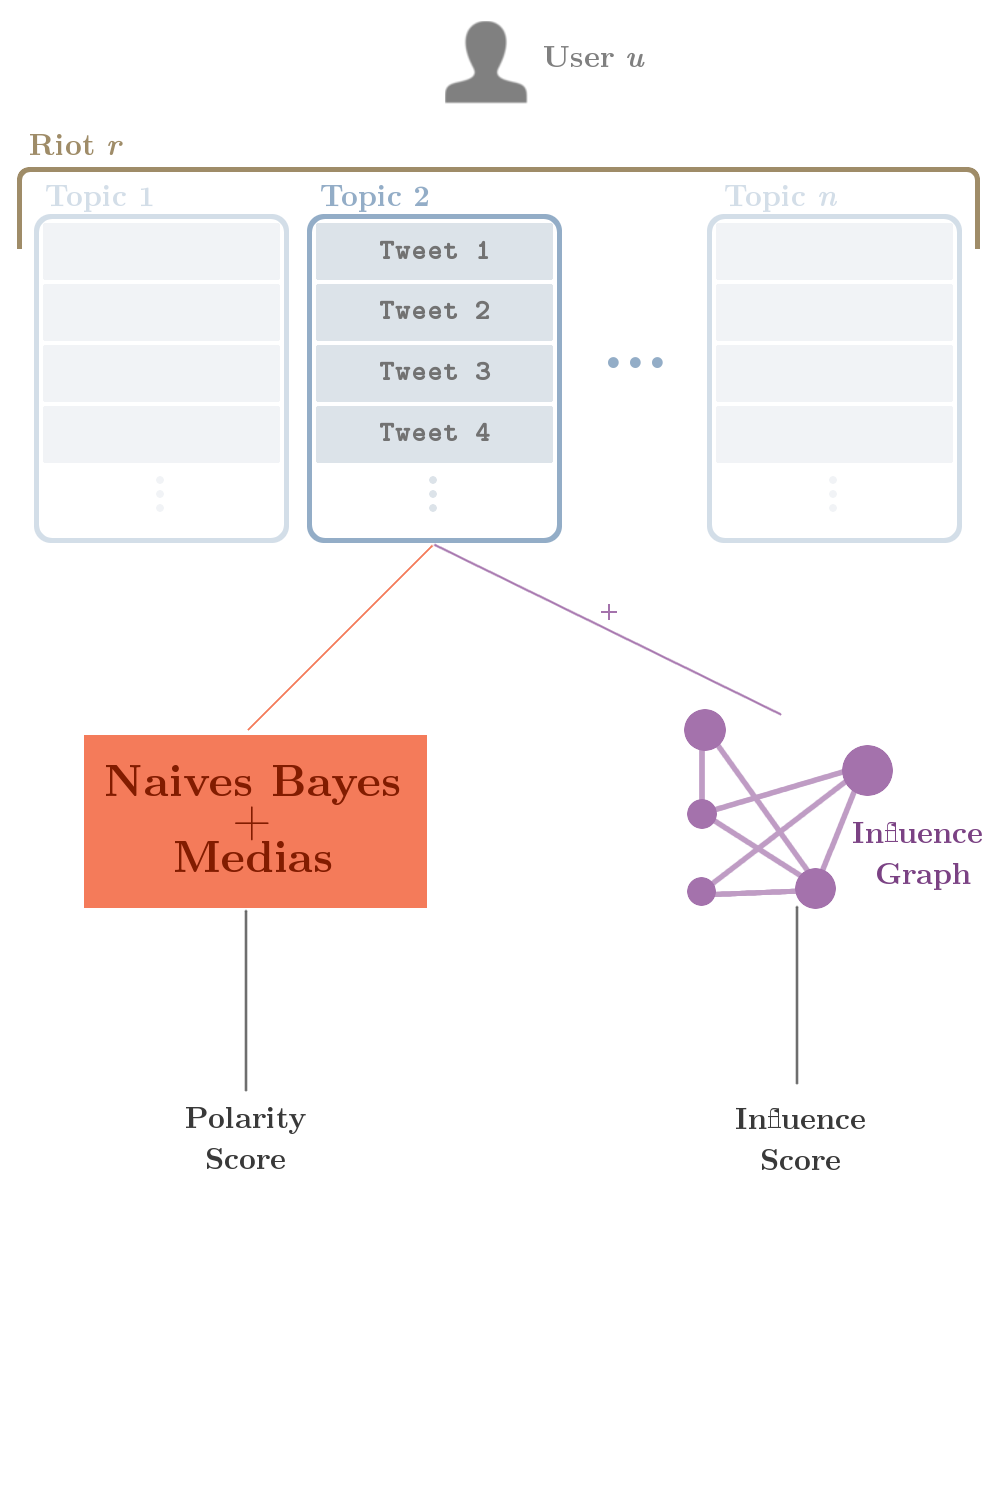
\includegraphics[width=0.95\textwidth]{images/diags/chain.png}
\caption{Unified model for the role vector computation}
\ref{unifiedModel}
\end{figure}


\newpage

\section{Experiments}
We conduct two experiments. First, we compute roles for single riots and then in the next part for two riots. 
\subsection{Roles during a riot}
On figure \ref{RolePlot14}, one can see the roles plotted after PCA and $t$-SNE reduction. The polarity is indicated with the color scale, and the influence is proportional to the dot sizes. 

On both figures, there is a clear between the informative users (light green dots) and the supportive users (dark green dots). Moreover, we can notice that the most influent users (big dots) are not grouped together but mixed with the others. The same results are obtained on figure \ref{RolePlot17}
\begin{figure}[H]
\begin{subfigure}[t]{0.5\textwidth}
\centering
\includegraphics[width=\textwidth]{images/plots/roles/pca_14_08.png}
\caption{PCA}
\label{Role14PCA}
\end{subfigure}
\hfill
\begin{subfigure}[t]{0.5\textwidth}
\centering
\includegraphics[width=\textwidth]{images/plots/roles/tsne_14_08.png}
\caption{$t$-SNE}
\label{Role14TSNE}
\end{subfigure}
\caption{Visualization for the roles on the August 14}
\label{RolePlot14}
\end{figure}

\begin{figure}[H]
\begin{subfigure}[t]{0.5\textwidth}
\centering
\includegraphics[width=\textwidth]{images/plots/roles/pca_17_08.png}
\caption{PCA}
\label{Role17PCA}
\end{subfigure}
\hfill
\begin{subfigure}[t]{0.5\textwidth}
\centering
\includegraphics[width=\textwidth]{images/plots/roles/tsne_17_08.png}
\caption{$t$-SNE}
\label{Role17TSNE}
\end{subfigure}
\caption{Visualization for the roles on the August 17}
\label{RolePlot17}
\end{figure}

We now put aside the concepts of influence and polarity and just analyze the disposition of the users on the plots. On figure \ref{Role14PCA} and \ref{Role14TSNE}, the users \texttt{ryanjreilly}, \texttt{yamiche}, \texttt{kodacohen} and \texttt{fox2now} are close together. By taking a look at their profile description, it turns out they are all journalists or news medias. 

In the same way, even if it is still compacted on the PCA plot, we notice that black personalities (i.e. people that may clearly defend black people in the Ferguson protests) like \texttt{antoniofrench}, \texttt{elonjames} and \texttt{wesleylowery}, as much as \texttt{youranonnews}, the account of the Anonymous hackers who also defended black people, appear in a different group on the plots (especially on the $t$-SNE plot).


However, on the figure \ref{RolePlot17}, we notice differences in the disposition between PCA and $t$-SNE. Indeed, on figure \ref{Role17PCA}, the users \texttt{youranonnews} and \texttt{ryanjreilly} are almost on the opposite, whereas they are very close on figure \label{Role17TSNE}.

We also perform the $k$-Nearest-Neighbors, an algorithm that returns the $k$ closest neighbors of a query point, with the Euclidean distance on the role vectors obtained from $t$-SNE. The results are shown on figure \ref{kNNRoleA}. On \ref{kNNRole14}, the query user is an activist hacker group, and we can see that the first and third users returns by the algorithm have described themselves as activists. In the same way, on the August 17, for the query \texttt{jonswaine} (journalist), one can see on figure \ref{kNNRole17} that there are five journalists or news related accounts and four of them are among the closest neighbors.

\vspace*{1cm}

\begin{figure}[H]
\begin{subfigure}[t]{0.5\textwidth}
\footnotesize
  \centering
\begin{tabular}{ccc}
\hline
Rank & \textbf{user} & \textbf{description} \\ \hline \hline
1 & edreggi & actor/activist \\ \hline
2 & 2chainzlyrics & / \\ \hline
3 & kathrynbruscobk & author/activist \\ \hline
4 & robertloerzel & author/journalist \\ \hline
5 & nickpistor & author/reporter \\ \hline
6 & fallongreen15 & / \\ \hline
7 & roricomics & author \\ \hline
8 & khatumofestival & / \\ \hline
9 & kim\_sutherland & / \\ \hline
10 & michaelcalhoun & journalist \\ \hline
\hline
\end{tabular}
\caption{August 14 with query user ``youranonnews"}
\label{kNNRole14}
\end{subfigure}
\hfill
\begin{subfigure}[t]{0.5\textwidth}
  \centering
  \footnotesize
\begin{tabular}{ccc}
\hline
Rank & \textbf{user} & \textbf{description} \\ \hline \hline
1 & chrishayestv & journalist \\ \hline
2 & plussone & activist \\ \hline
3 & laureldavilacpa & radio commentator \\ \hline
4 & twitchyteam & news software \\ \hline
5 & michaelcalhoun & journalist \\ \hline
6 & fallongreen15 & / \\ \hline
7 & \_nealanae & / \\ \hline
8 & wesknuckle & / \\ \hline
9 & 2chainzlyrics & / \\ \hline
10 & nickpistor & journalist \\ \hline
\hline
\end{tabular}
\caption{August 17 with query user ``jonswaine"}
\label{kNNRole17}
\end{subfigure}
\caption{Users returned with a $k$-NN search on the $t$-SNE values for a specified}
\label{kNNRoleA}
\end{figure}

\newpage

\subsection{Role similarity between $m$ riots}

\begin{figure}[H]
\centering
\includegraphics[width=\textwidth]{images/plots/roles/tsne_inter_14_17_08.png}
\caption{$t$-SNE plot of the roles on the August 14th and 17th}
\label{}
\end{figure}


\begin{figure}[H]
  \centering
\begin{tabular}{ccc}
\hline
Rank & \textbf{user} & \textbf{description} \\ \hline \hline
1 & soulrevision & activist \\ \hline
2 & copwatchnews & activists news \\ \hline
3 & breaking3zero & news website \\ \hline
4 & allthenewsisnow & news website \\ \hline
5 & ryanjreilly & journalist \\ \hline
6 & realtimehack & / \\ \hline
7 & haiku\_rs & / \\ \hline
8 & washingtonpost & news website \\ \hline
9 & monaeltahawy & author/journal columnist \\ \hline
10 & youranoncentral & hackers account \\ \hline
\hline
\end{tabular}
\caption{Users returned with a $k$-NN search for the query user ``pzfeed"}
\end{figure}

\chapter{Related work}
\section{Crisis informatics}
Crisis events have been a topic of study over the past few years in computer science with the progressive use of social medias in the whole world. This studies lead to a new field called \emph{crisis informatics}.

\cite{vieweg2015expect} analyzes data from 26 crisis events of several types (like floods, earthquakes, wildfires, shootings, bombings etc.) and makes a transversal study of the information types and sources shared on Twitter. The study shows that :
\begin{enumerate}
\item even if such events happen regularly, each crisis remains unique, even two disasters of the same type occuring in the same country.
\item human-induced crises (riots, shootings..) tend to be more similar to each other than to natural disasters.
\end{enumerate}

\cite{imran2013extracting} descibes a method for processing messages from social medias in order to extract useful information. The proposed system uses machine learning methods like Naive Bayes to classify relevant messages and obtains good accuracy results.

\cite{mendoza2010twitter} studies Twitter messages after the 2010 Chile earthquake. Among other things, this paper analyzes the propagation of false and true rumors and shows that false rumors can be detected. Indeed, these messages tend to be more called into question, and as a consequence machine learning can target them.

Finally, \cite{imran2014processing} is a state of the art about processing social medias messages during crisis events. It describes all the steps, which are in the order : data acquisition, preprocessing, event detection, event tracking, clustering / classification, information extraction, summarization, semantic enrichment and ontologies. For each section, the paper describes the existing techniques, their results, and the main relevant papers.
\newpage
\section{Riots}
There are already some papers existing about social medias and riots.

\subsection{London riots}

The 2011 London riots lead to several study over the past few years. 
\cite{procter2013reading} analyzed by what kind of actor (media, celebrity, activist etc.) was used Twitter during that period. The paper also focuses on rumors, how they spread during the riots and how they can be called into question.
\cite{tonkin2012twitter} try 

\newpage

\chapter{Conclusion}
\section{Summary}
In this project we have introduced a framework for analyzing roles of users during a riot. The dataset contains messages from Twitter during the 2014 US Ferguson protests.\\[2pt]

In chapter 3, we first perform some preprocessing on the data. Then, we extract topics from a riot by comparing two techniques : $k$-means and Latent Dirichlet Allocation. After experimenting, we choose to select the second method.\\[2pt]

In chapter 4, we focus on the content of the tweets. After having established a classification of types, we train and test a Naive Bayes classifier to predict if a tweet is either supportive or informative about the riot. We also study the medias shared by users in order to improve our classifier and in the end we define and compute user polarity score.\\[2pt]

In chapter 5, we perform graph analysis on the hashtags and users and we visualize these networks through examples. We also define and compute user influence score with degree centrality and Page Rank. We choose to keep for the next chapter the Page Rank method, as it is more realistic. \\[2pt]

Finally, we define the role of a user during a riot (or several) as being the feature vector of its polarity and influence scores for each topic. We perform dimension reduction with PCA and $t$-SNE for visualization purpose and neighbors research. Through experiments, we show how users with the same job (for example journalists or activists) are grouped together.

\newpage
\section{Future work}
In this section we identify some future work tracks to improve our framework.

Firstly, it is possible to perform more in-depth Natural Language Processing analysis in the begining. Indeed, it would be interesting to add a lemming or stemming step in section 3.2. These processing would allow to consider for example words as \emph{riot} and \emph{riot\underline{s}} to be represented as the same, as much as for the words \emph{loot\underline{ing}} and \emph{loot\underline{ed}}. In addition to reducing the vocabulary size, it may improve the model accuracy in section 4.2.2. We can also think about create a lexicon specific to riots in order to detect and classify better informative and supportive tweets.

Secondly, our model remains quite simple, as it only consider two features : the \emph{influence} and the \emph{polarity}. It may also be a good track to define new features to characterize the role of a user. For example, it would be possible to use the hashtags communities found in 5.2.2.

Finally, it would be necessary to perform more exhaustive tests on our framework by playing with the different parameter. For example, it would be interesting to try with a different number of topics or a different vocabulary size. Moreover, tests on more riots days should be performed to identify strengths and weaknesses of our model.

\bibliographystyle{apalike}
\bibliography{biblio}

\end{document}
